%  template.tex for Biometrics papers
%
%  This file provides a template for Biometrics authors.  Use this
%  template as the starting point for creating your manuscript document.
%  See the file biomsample.tex for an example of a full-blown manuscript.

%  ALWAYS USE THE referee OPTION WITH PAPERS SUBMITTED TO BIOMETRICS!!!
%  You can see what your paper would look like typeset by removing
%  the referee option.  Because the typeset version will be in two
%  columns, however, some of your equations may be too long. DO NOT
%  use the \longequation option discussed in the user guide!!!  This option
%  is reserved ONLY for equations that are impossible to split across 
%  multiple lines; e.g., a very wide matrix.  Instead, type your equations 
%  so that they stay in one column and are split across several lines, 
%  as are almost all equations in the journal.  Use a recent version of the
%  journal as a guide. 
%  
%\documentclass[useAMS,usenatbib, referee]{biom}
\documentclass[useAMS, usenatbib]{biom}
%
%  If your system does not have the AMS fonts version 2.0 installed, then
%  remove the useAMS option.
%
%  useAMS allows you to obtain upright Greek characters.
%  e.g. \umu, \upi etc.  See the section on "Upright Greek characters" in
%  this guide for further information.
%
%  If you are using AMS 2.0 fonts, bold math letters/symbols are available
%  at a larger range of sizes for NFSS release 1 and 2 (using \boldmath or
%  preferably \bmath).
% 
%  Other options are described in the user guide. Here are a few:
% 
%  -  If you use Patrick Daly's natbib  to cross-reference your 
%     bibliography entries, use the usenatbib option
%
%  -  If you use \includegraphics (graphicx package) for importing graphics
%     into your figures, use the usegraphicx option
% 
%  If you wish to typeset the paper in Times font (if you do not have the
%  PostScript Type 1 Computer Modern fonts you will need to do this to get
%  smoother fonts in a PDF file) then uncomment the next line
%  \usepackage{Times}
\usepackage[tbtags]{amsmath}

%Following 3 lines for Tikz
\usepackage{tikz}
\usepackage{tikzscale}
\usepackage{graphicx}
\usepackage{url}
\usetikzlibrary{shapes.geometric, arrows, positioning}
%%%%% PLACE YOUR OWN MACROS HERE %%%%%

\def\bSig\mathbf{\Sigma}
\newcommand{\VS}{V\&S}
\newcommand{\tr}{\mbox{tr}}

\DeclareMathOperator{\argmax}{arg\,max}


\tikzstyle{startstop_big} = [rectangle, rounded corners, minimum width=3cm, minimum height=1cm,text centered, draw=black,text width = 8.5cm, fill=red!30]
\tikzstyle{startstop} = [rectangle, rounded corners, minimum width=3cm, minimum height=1cm,text centered, draw=black,text width = 5cm, fill=red!30]
\tikzstyle{io} = [trapezium, trapezium left angle=70, trapezium right angle=110, minimum width=2cm, minimum height=1cm, text centered, draw=black, fill=blue!30]
\tikzstyle{process} = [rectangle, minimum width=3cm, minimum height=1cm, text centered, text width = 3cm, draw=black, fill=orange!30]
\tikzstyle{process_wide_3pt5cm} = [rectangle, minimum width=3cm, minimum height=1cm, text centered, text width = 3.5cm, draw=black, fill=orange!30]
\tikzstyle{process_wide_4cm} = [rectangle, minimum width=3cm, minimum height=1cm, text centered, text width = 4cm, draw=black, fill=orange!30]
\tikzstyle{process_wide_4pt5cm} = [rectangle, minimum width=3cm, minimum height=1cm, text width = 4.5cm, draw=black, fill=orange!30]
\tikzstyle{process_wide_5cm} = [rectangle, minimum width=3cm, minimum height=1cm, text width = 5cm, draw=black, fill=orange!30]
\tikzstyle{decision} = [diamond, minimum width=1cm, minimum height=1cm,text centered,text width = 2.25cm, draw=black, fill=green!30]
\tikzstyle{arrow} = [thick,->,>=stealth]


%  The rotating package allows you to have tables displayed in landscape
%  mode.  The rotating package is NOT included in this distribution, but
%  can be obtained from the CTAN archive.  USE OF LANDSCAPE TABLES IS
%  STRONGLY DISCOURAGED -- create landscape tables only as a last resort if
%  you see no other way to display the information.  If you do do this,
%  then you need the following command.

%\usepackage[figuresright]{rotating}

%%%%%%%%%%%%%%%%%%%%%%%%%%%%%%%%%%%%%%%%%%%%%%%%%%%%%%%%%%%%%%%%%%%%%

%  Here, place your title and author information.  Note that in 
%  use of the \author command, you create your own footnotes.  Follow
%  the examples below in creating your author and affiliation information.
%  Also consult a recent issue of the journal for examples of formatting.

\title[Personalized Schedules for Surveillance of Low Risk Prostate Cancer Patients]
{Personalized Schedules for Surveillance of Low Risk Prostate Cancer Patients}

%  Here are examples of different configurations of author/affiliation
%  displays.  According to the Biometrics style, in some instances,
%  the convention is to have superscript *, **, etc footnotes to indicate 
%  which of multiple email addresses belong to which author.  In this case,
%  use the \email{ } command to produce the emails in the display.

%  In other cases, such as a single author or two authors from 
%  different institutions, there should be no footnoting.  Here, use
%  the \emailx{ } command instead. 

%  The examples below corrspond to almost every possible configuration
%  of authors and may be used as a guide.  For other configurations, consult
%  a recent issue of the the journal.

%  Single author -- USE \emailx{ } here so that no asterisk footnoting
%  for the email address will be produced.

%\author{John Author\emailx{email@address.edu} \\
%Department of Statistics, University of Warwick, Coventry CV4 7AL, U.K.}

%  Two authors from the same institution, with both emails -- use
%  \email{ } here to produce the asterisk footnoting for each email address

%\author{John Author$^{*}$\email{author@address.edu} and
%Kathy Authoress$^{**}$\email{email2@address.edu} \\
%Department of Statistics, University of Warwick, Coventry CV4 7AL, U.K.}

%  Exactly two authors from different institutions, with both emails  
%  USE \emailx{ } here so that no asterisk footnoting for the email address
%  is produced.

%\author
%{John Author\emailx{author@address.edu} \\
%Department of Statistics, University of Warwick, Coventry CV4 7AL, U.K. 
%\and
%Kathy Author\emailx{anotherauthor@address.edu} \\
%Department of Biostatistics, University of North Carolina at Chapel Hill, 
%Chapel Hill, North Carolina, U.S.A.}

%  Three or more authors from same institution with all emails displayed
%  and footnoted using asterisks -- use \email{ } 

%\author{John Author$^*$\email{author@address.edu}, 
%Jane Author$^{**}$\email{jane@address.edu}, and 
%Dick Author$^{***}$\email{dick@address.edu} \\
%Department of Statistics, University of Warwick, Coventry CV4 7AL, U.K}

%  Three or more authors from same institution with one corresponding email
%  displayed

%\author{Anirudh Tomer$^*$\email{atomer@erasmusmc.nl}, 
%Jane Author, and Dimitris Rizopoulos \\
%Department of Statistics, University of Latex, Coventry CV4 7AL, U.K}

%  Three or more authors, with at least two different institutions,
%  more than one email displayed 

%\author{John Author$^{1,*}$\email{author@address.edu}, 
%Kathy Author$^{2,**}$\email{anotherauthor@address.edu}, and 
%Wilma Flinstone$^{3,***}$\email{wilma@bedrock.edu} \\
%$^{1}$Department of Statistics, University of Warwick, Coventry CV4 7AL, U.K \\
%$^{2}$Department of Biostatistics, University of North Carolina at 
%Chapel Hill, Chapel Hill, North Carolina, U.S.A. \\
%$^{3}$Department of Geology, University of Bedrock, Bedrock, Kansas, U.S.A.}

%  Three or more authors with at least two different institutions and only
%  one email displayed

\author{Anirudh Tomer$^{1,*}$\email{atomer@erasmusmc.nl}, 
Daan Nieboer$^{2}$, 
Monique J. Roobol$^3$, \\
\textbf{Ewout W. Steyerberg}$^{\bmath{2, 4}}$, 
\textbf{and Dimitris Rizopoulos}$^{\bmath{1}}$ \\ \\
$^{1}$Department of Biostatistics, Erasmus University Medical Center, the Netherlands \\
$^{2}$Department of Public Health, Erasmus University Medical Center, the Netherlands \\
$^{3}$Department of Urology, Erasmus University Medical Center, the Netherlands \\
$^{4}$Department Medical Statistics and Bioinformatics, Leiden University Medical Center, the Netherlands}


\begin{document}

%  This will produce the submission and review information that appears
%  right after the reference section.  Of course, it will be unknown when
%  you submit your paper, so you can either leave this out or put in 
%  sample dates (these will have no effect on the fate of your paper in the
%  review process!)

\date{{\it Received October} 0000. {\it Revised February} 0000.  {\it
Accepted March} 0000.}

%  These options will count the number of pages and provide volume
%  and date information in the upper left hand corner of the top of the 
%  first page as in published papers.  The \pagerange command will only
%  work if you place the command \label{firstpage} near the beginning
%  of the document and \label{lastpage} at the end of the document, as we
%  have done in this template.

%  Again, putting a volume number and date is for your own amusement and
%  has no bearing on what actually happens to your paper!  

\pagerange{\pageref{firstpage}--\pageref{lastpage}} 
\volume{00}
\pubyear{0000}
\artmonth{December}

%  The \doi command is where the DOI for your paper would be placed should it
%  be published.  Again, if you make one up and stick it here, it means 
%  nothing!

\doi{10.1111/j.1541-0420.2005.00454.x}

%  This label and the label ``lastpage'' are used by the \pagerange
%  command above to give the page range for the article.  You may have 
%  to process the document twice to get this to match up with what you 
%  expect.  When using the referee option, this will not count the pages
%  with tables and figures.  

\label{firstpage}

%  put the summary for your paper here

%\begin{abstract}
%This is the summary for this paper.
%\end{abstract}

% !TEX root =  ../main_manuscript.tex 
\begin{abstract}
\texttt{Background}: Prostate cancer active surveillance (AS) patients undergo repeat biopsies. Active treatment is advised when biopsy Gleason grade group~$\geq$~2 (\textit{upgrading}). Many patients never experience upgrading, yet undergo biopsies frequently. Personalized biopsy decisions based on upgrading-risk may reduce patient burden.\\

\texttt{Objective}: Develop a risk prediction model and web-application to assist patients/doctors in personalized biopsy decisions.\\

\texttt{Design, Setting, and Participants}: Model development: world's largest AS study PRIAS, 7813 patients, 1134 experienced upgrading; External validation: largest five cohorts of Movember Foundation's GAP3 database (${>20,000}$ patients, 27 centers worldwide); Data: repeat prostate-specific antigen (PSA) and biopsy Gleason grade.\\

\texttt{Outcome Measurements, and Statistical Analysis}: A Bayesian joint model fitted to the PRIAS dataset. This model was validated in GAP3 cohorts using risk prediction error, calibration, area under ROC (AUC). Model and personalized biopsy schedules based on predicted risks were implemented in a web-application.\\

\texttt{Results and Limitations}: Cause-specific cumulative upgrading-risk at year five of follow-up: 35\% in PRIAS, at most 50\% in GAP3 cohorts. PRIAS based model: PSA velocity was a stronger predictor of upgrading (Hazard~Ratio:~2.47, 95\%CI:~1.93--2.99) than PSA value (Hazard~Ratio:~0.99, 95\%CI:~0.89--1.11). Validation: Moderate AUC (0.55--0.75) in PRIAS and GAP3 cohorts. Moderate prediction error (0.1--0.3) in GAP3 cohorts where impact of PSA value and velocity on upgrading-risk was similar to PRIAS, but large (0.3--0.45) otherwise. Recalibration advised for external cohorts.\\

\texttt{Conclusions}: We successfully developed and validated a model for predicting upgrading-risk, and providing risk-based personalized biopsy decisions, in prostate cancer AS. The model made available via a web-application enables shared decision making of biopsy schedules by comparing fixed and personalized schedules on total biopsies and expected time delay in detecting upgrading.\\

\texttt{Patient Summary}: Personalized prostate biopsies are a novel alternative to fixed one-size-fits-all schedules. The underlying statistical models are made available through a user-friendly web-application and may help to reduce unnecessary prostate biopsies while maintaining cancer control.
\end{abstract}

%  Please place your key words in alphabetical order, separated
%  by semicolons, with the first letter of the first word capitalized,
%  and a period at the end of the list.
%

\begin{keywords}
 Active surveillance; Biopsy; Joint models; Personalized medicine; Prostate Cancer
\end{keywords}

%  As usual, the \maketitle command creates the title and author/affiliations
%  display 

\maketitle

%  If you are using the referee option, a new page, numbered page 1, will
%  start after the summary and keywords.  The page numbers thus count the
%  number of pages of your manuscript in the preferred submission style.
%  Remember, ``Normally, regular papers exceeding 25 pages and Reader Reaction 
%  papers exceeding 12 pages in (the preferred style) will be returned to 
%  the authors without review. The page limit includes acknowledgements, 
%  references, and appendices, but not tables and figures. The page count does 
%  not include the title page and abstract. A maximum of six (6) tables or 
%  figures combined is often required.''

%  You may now place the substance of your manuscript here.  Please use
%  the \section, \subsection, etc commands as described in the user guide.
%  Please use \label and \ref commands to cross-reference sections, equations,
%  tables, figures, etc.
%
%  Please DO NOT attempt to reformat the style of equation numbering!
%  For that matter, please do not attempt to redefine anything!

% !TEX root =  ../main_manuscript.tex 
\section{Introduction}
Patients with low- and very low-risk screening-detected localized prostate cancer are usually advised active surveillance (AS) instead of immediate radical treatment~\citep{briganti2018active}. In AS, cancer progression is routinely monitored via prostate-specific antigen (PSA), digital rectal examination, and repeat biopsies. Among these, the strongest indicator of cancer-related outcomes is the biopsy Gleason grade~\citep{epsteinGG2014}. When the Gleason grade increases from grade~1 (Gleason 3+3) to 2 (Gleason 3+4) or higher, called \textit{reclassification}, patients are commonly advised curative treatment~\citep{bul2013active}.

\begin{figure}
\centerline{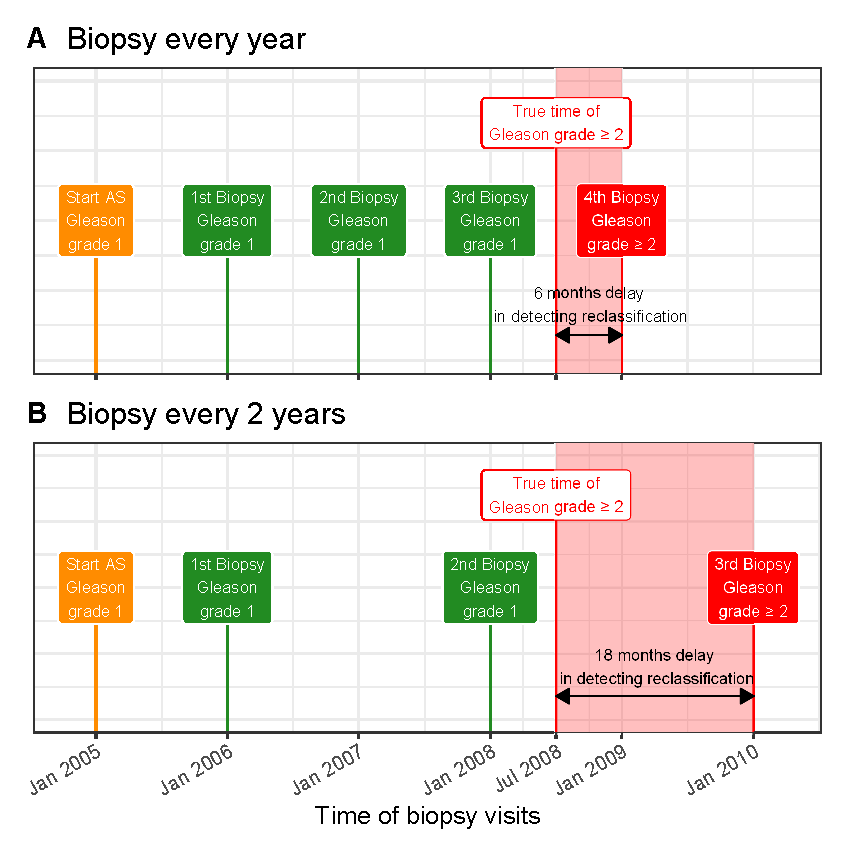
\includegraphics[width=\columnwidth]{images/delay_explanation.eps}}
\caption{\textbf{Trade-off between the number of biopsies and time delay in detecting reclassification (Increase in Gleason grade from 1 to 2 or higher):} The true time of reclassification for the patient in this figure is July 2008. When biopsies are scheduled annually (\textbf{Panel~A}), reclassification is detected in January 2009 with a time delay of six months, and a total of four biopsies are scheduled. When biopsies are scheduled biennially (\textbf{Panel~B}) reclassification is detected in January 2010 with a time delay of 18 months, and a total of three biopsies are scheduled. Since biopsies are conducted periodically, the time of reclassification is observed as an interval. For example, between Jan~2008--Jan~2009 in \textbf{Panel~A} and between Jan~2008--Jan~2010 in \textbf{Panel~B}.}
\label{fig:delay_explanation}
\end{figure}

Biopsies are conducted periodically. Consequently, reclassification is always detected with a time delay (Figure~\ref{fig:delay_explanation}). For detecting reclassification timely, many AS programs schedule fixed and frequent biopsies (e.g.,~annually) for all patients~\citep{nieboer2018active,loeb2014heterogeneity}. However, this also leads to many unnecessary biopsies in slow/non-progressing patients. Biopsies are invasive, painful and prone to medical complications. Thus, biopsy burden and patient non-compliance to frequent biopsies~\citep{bokhorst2015compliance} has raised concerns regarding the optimal biopsy schedule~\citep{inoue2018comparative, bratt2013study}. To this end, infrequent schedules such as biennial biopsies have been proposed as an alternative~\citep{inoue2018comparative,de2017estimating}. Although, biennial biopsies may still lead to five unnecessary biopsies over ten years (current study period of large AS programs) for slow/non-progressing patients. A promising alternative to fixed and frequent biopsies is personalized biopsy schedules based on the patient-specific risk of reclassification (Figure~\ref{fig:riskBasedExample}).

\begin{figure}
\centerline{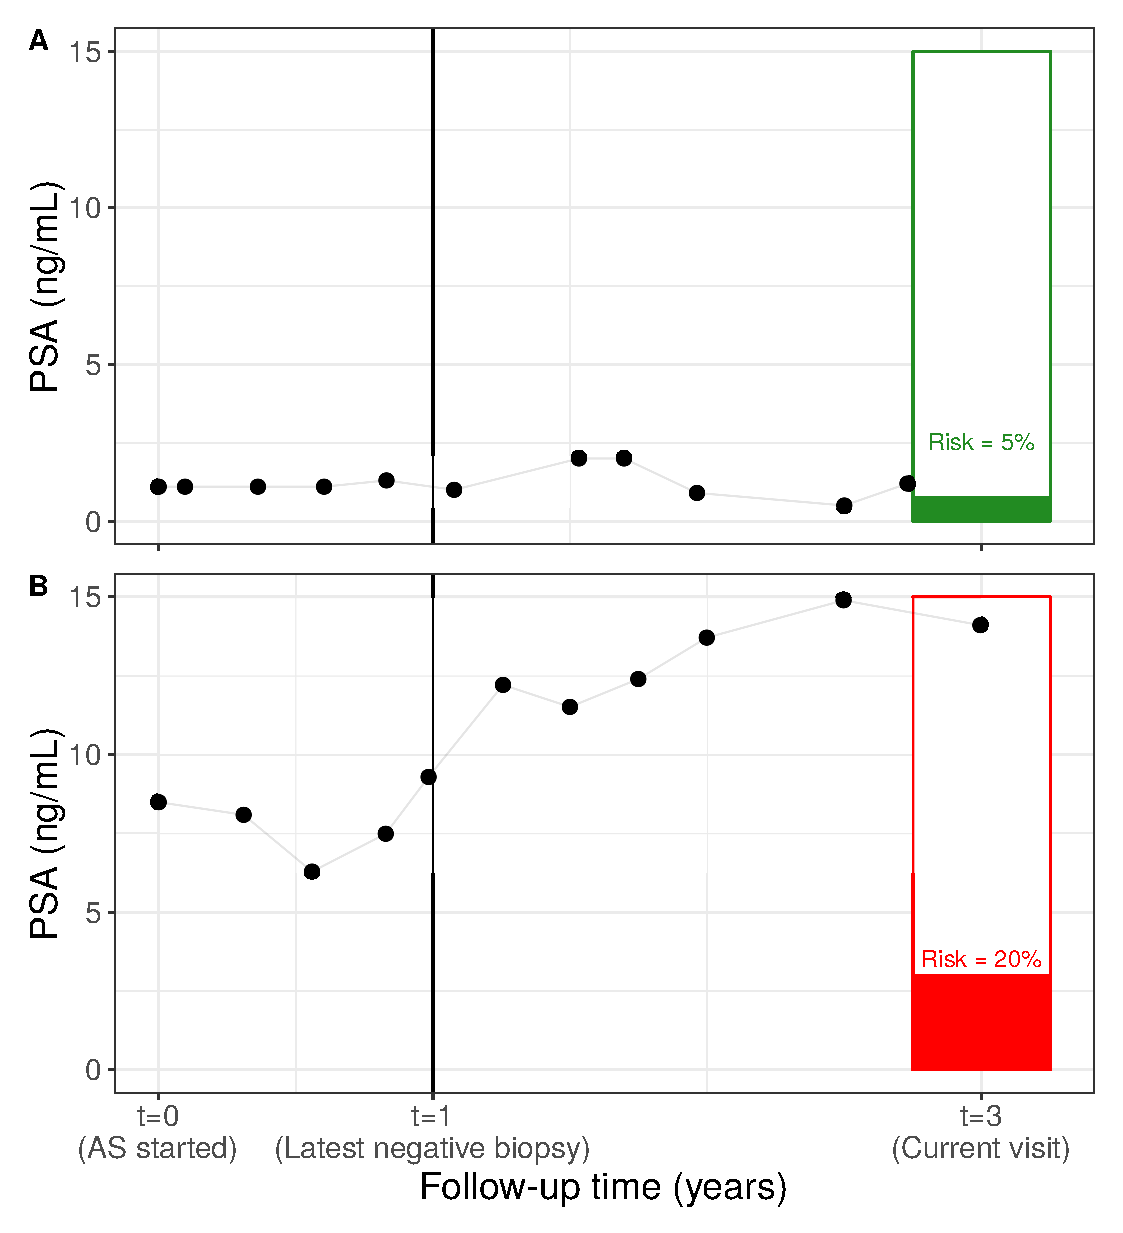
\includegraphics[width=\columnwidth]{images/riskBasedExample.eps}}
\caption{\textbf{Motivation for personalized risk-based decisions of biopsy}: Patient~A (\textbf{Panel~A}) and B (\textbf{Panel~B}) had their latest biopsy at year one of follow-up (green vertical line). Patient~A's prostate-specific antigen (PSA) profile remained stable until his current visit at year three, whereas patient~B's profile has shown a rise. Consequently, patient~B's estimated cumulative risk of reclassification at the current visit (year three) is higher than that of patient~A. This makes patient~B a more suitable candidate for biopsy than Patient~A. Risk estimates in this figure are only illustrative.}
\label{fig:riskBasedExample}
\end{figure}

The first challenge in developing personalized biopsy schedules is consolidating accumulated patient data (e.g., PSA, previous biopsy results) into risk estimates for reclassification. Existing calculators for risk of reclassification~\citep{partin1993use,makarov2007updated} use only the latest PSA measurement of a patient. In contrast, we intend to utilize all repeated measurements of PSA, previous biopsy results, and baseline characteristics of a patient. To this end, a suitable model is the joint model for time-to-event and longitudinal data~\citep{tomer2019, coley2017prediction,rizopoulos2012joint}. A joint model predicts risk of reclassification in a personalized manner. A subsequent challenge however, is translating risks into clinical decisions. For example, a 10\% risk of reclassification can be perceived high/low depending upon the patient age. Patients may also weigh risks of reclassification with the potential \textit{consequences} of another biopsy. Two relevant \textit{consequences} of biopsies (Figure~\ref{fig:delay_explanation}) are the timing and total number of biopsies (burden), and the time delay in detecting reclassification (smaller is beneficial). The relative importance of these \textit{consequences} can vary between the patients, and also over the follow-up period for the same patient.

The goal of this work was to assist patients and doctors in making better decisions of biopsies than fixed and frequent biopsies. For this purpose, we developed a web-application that gives patients their current and future risk of reclassification. It also suggests them risk-based personalized schedules of biopsies. For each biopsy schedule, be it fixed or personalized, the web-application provides expected \textit{consequences} of following it. Thus, patients can compare schedules before making a decision. The web-application uses a prediction joint model fitted to the world's largest AS dataset, PRIAS~\citep{bul2013active}. We externally validated this model in five largest AS cohorts of the GAP3 database \citep{gap3_2018}. Thus, the web-application can be used by a large number of patients worldwide.
% !TEX root =  main_manuscript.tex 
\section{Joint Model for Time-to-Event and Longitudinal Outcomes}
\label{sec : jm_framework}
We start with a short introduction of the joint modeling framework we will use in our following developments. Let $T_i^*$ denote the true GR time for the $i$-th patient and let $S$ be the schedule of his biopsies. Let the vector of the time of biopsies be denoted by $T_i^S = \{T^S_{i0}, T^S_{i1}, \ldots, T^S_{i{N_i^S}}; T^S_{ij} < T^S_{ik}, \forall j<k\}$, where $N_i^S$ are the total number of biopsies conducted. Because biopsy schedules are periodical, $T_i^*$ cannot be observed directly and it is only known to fall in an interval $l_i < T_i^* \leq r_i$, where $l_i = T^S_{i{N_i^S - 1}}, r_i = T^S_{i{N_i^S}}$ if GR is observed, and $l_i = T^S_{i{N_i^S}}, r_i=\infty$ if GR is not observed yet. Further let $\bmath{y}_i$ denote the $n_i \times 1$ vector of PSA levels for the $i$-th patient. For a sample of $n$ patients the observed data is denoted by $\mathcal{D}_n = \{l_i, r_i, \bmath{y}_i; i = 1, \ldots, n\}$.

The longitudinal outcome of interest, namely PSA level, is continuous in nature and thus to model it the joint model utilizes a linear mixed effects model (LMM) of the form:
\begin{equation*}
\begin{split}
y_i(t) &= m_i(t) + \varepsilon_i(t)\\
&=\bmath{x}_i^T(t) \bmath{\beta} + \bmath{z}_i^T(t) \bmath{b}_i + \varepsilon_i(t),
\end{split}
\end{equation*}
where $\bmath{x}_i(t)$ and $\bmath{z}_i(t)$ denote the row vectors of the design matrix for fixed and random effects, respectively. The fixed and random effects are denoted by $\bmath{\beta}$ and $\bmath{b}_i$, respectively. The random effects are assumed to be normally distributed with mean zero and $q \times q$ covariance matrix $\bmath{D}$. The true and unobserved, error free PSA level at time $t$ is denoted by $m_i(t)$. The error $\varepsilon_i(t)$ is assumed to be t-distributed with three degrees of freedom and scale $\sigma$ (see Web Appendix C.1), and is independent of the random effects $\bmath{b}_i$.

To model the effect of PSA on hazard of GR, joint models utilize a relative risk sub-model. The hazard of GR for patient $i$ at any time point $t$, denoted by $h_i(t)$, depends on a function of subject specific linear predictor $m_i(t)$ and/or the random effects:
\begin{align*}
h_i(t \mid \mathcal{M}_i(t), \bmath{w}_i) &= \lim_{\Delta t \to 0} \frac{\mbox{Pr}\big\{t \leq T^*_i < t + \Delta t \mid T^*_i \geq t, \mathcal{M}_i(t), \bmath{w}_i\big\}}{\Delta t}\\
&=h_0(t) \exp\big[\bmath{\gamma}^T\bmath{w}_i + f\{\mathcal{M}_i(t), \bmath{b}_i, \bmath{\alpha}\}\big], \quad t>0,
\end{align*}
where $\mathcal{M}_i(t) = \{m_i(v), 0\leq v \leq t\}$ denotes the history of the underlying PSA levels up to time $t$. The vector of baseline covariates is denoted by $\bmath{w}_i$, and $\bmath{\gamma}$ are the corresponding parameters. The function $f(\cdot)$ parametrized by vector $\bmath{\alpha}$ specifies the functional form of PSA levels \citep{brown2009assessing,rizopoulos2012joint,taylor2013real,rizopoulos2014bma} that is used in the linear predictor of the relative risk model. Some functional forms relevant to the problem at hand are the following: 
\begin{eqnarray*}
\left \{
\begin{array}{l}
f\{\mathcal{M}_i(t), \bmath{b}_i, \bmath{\alpha}\} = \alpha m_i(t),\\
f\{\mathcal{M}_i(t), \bmath{b}_i, \bmath{\alpha}\} = \alpha_1 m_i(t) + \alpha_2 m'_i(t),\quad \text{with}\  m'_i(t) = \frac{\rmn{d}{m_i(t)}}{\rmn{d}{t}}.\\
\end{array}
\right.
\end{eqnarray*}
These formulations of $f(\cdot)$ postulate that the hazard of GR at time $t$ may be associated with the underlying level $m_i(t)$ of the PSA at $t$, or with both the level and velocity $m'_i(t)$ of the PSA at $t$. Lastly, $h_0(t)$ is the baseline hazard at time $t$, and is modeled flexibly using P-splines. The detailed specification of the baseline hazard, and parameter estimation using the Bayesian approach are presented in Web Appendix A of the supplementary material.
% !TEX root =  ../pers_schedules.tex 
\section{Personalized schedules for repeat biopsies}
\label{sec : pers_sched_approaches}
Once a joint model for GR and PSA levels is obtained, the next step is to use it to create personalized schedules for biopsies. To elucidate personalized schedules, let us assume that a personalized schedule is to be created for a new patient $j$, who is not present in the original sample of patients $\mathcal{D}_n$. Further let us assume that this patient did not have a GR at his last biopsy performed at time $t$, and that the PSA levels are available up to a time point $s$. The goal is to find the optimal time $u \geq \mbox{max}(t,s)$ of the next biopsy. 

% !TEX root =  ../main.tex 

\subsection{Posterior predictive distribution for time to GR}
\label{subsec : ppd_time_to_GR}
Let $\mathcal{Y}_j(s)$ denote the history of PSA levels taken up to time $s$ for patient $j$. The information from PSA history and repeat biopsies is manifested by the posterior predictive distribution $g(T^*_j)$, given by (conditioning on baseline covariates $\boldsymbol{w}_i$ is dropped for notational simplicity hereafter):
\begin{equation}
\label{eq : dyn_dist_fail_time}
\begin{split}
g(T^*_j) &= p\big(T^*_j \mid T^*_j > t, \mathcal{Y}_j(s), \mathcal{D}_n\big)\\
&= \int p\big(T^*_j \mid T^*_j > t, \mathcal{Y}_j(s), \boldsymbol{\theta}\big) p\big(\boldsymbol{\theta} \mid \mathcal{D}_n\big) \rmn{d} \boldsymbol{\theta}\\
&= \int \int p\big(T^*_j \mid T^*_j > t, \boldsymbol{b_j}, \boldsymbol{\theta}\big) p\big(\boldsymbol{b}_j \mid T^*_j>t, \mathcal{Y}_j(s), \boldsymbol{\theta}\big)p\big(\boldsymbol{\theta} \mid \mathcal{D}_n\big) \rmn{d} \boldsymbol{b}_j \rmn{d} \boldsymbol{\theta}
\end{split}
\end{equation}
The posterior predictive distribution depends on the observed longitudinal history via the random effects $\boldsymbol{b_j}$. The posterior distribution of the parameters $\boldsymbol{\theta}$, denoted by $p(\boldsymbol{\theta} \mid \mathcal{D}_n)$ is obtained as in Section \ref{subsec : jm_param_estimation_bayesian}.
% !TEX root =  ../pers_schedules.tex 

\subsection{Loss functions}
\label{subsec : loss_functions}
To find the time $u$ of next biopsy, we use principles from statistical decision theory in a Bayesian setting \citep{bergerDecisionTheory,robertBayesianChoice}. More specifically, we propose to choose future biopsy time $u$ by minimizing the posterior expected loss $E_g\big[L\{T^*_j, u\}\big]$, where the expectation is taken w.r.t. the PPD $g(T^*_j)$. The former is given by:
\begin{equation*}
E_g\big[L\{T^*_j, u\}\big] = \int_t^\infty L\{T^*_j, u\} p\big(T^*_j \mid T^*_j > t, \mathcal{Y}_j(s), \mathcal{D}_n\big) \rmn{d} T^*_j
\end{equation*}
Various loss functions $L\{T^*_j, u\}$ have been proposed in literature \citep{robertBayesianChoice}. The ones we utilize, and the corresponding motivations are presented next.

\subsubsection{Expected and median time of GR}
\label{subsubsec : exp_median_fail_time}
One of the reasons, patients did not comply with the existing PRIAS schedule was \textquoteleft complications on a previous biopsy\textquoteright. Therefore, it makes sense to have as less biopsies as possible. In the ideal case only 1 biopsy, performed at the exact time of GR is sufficient. Hence, neither a time which overshoots the true GR time $T^*_j$, nor a time which undershoots is preferred. In this regard, the squared loss function $L\{T^*_j, u\} = (T^*_j - u)^2$ and absolute loss function $L\{T^*_j, u\} = \left|{T^*_j - u}\right|$ have the properties that the posterior expected loss is symmetric on both sides of $T^*_j$. Secondly, both loss functions have well known solutions available. The posterior expected loss for the squared loss function is given by:
\begin{equation}
\label{eq : posterior_squared_loss}
\begin{split}
E_g\big[L\{T^*_j, u\}\big] &= E_g\big[\{T^*_j - u\}^2\big]\\
&=E_g\big[\{T^*_j\}^2\big] + u^2 -2uE_g[T^*_j]
\end{split}
\end{equation}
The posterior expected loss in (\ref{eq : posterior_squared_loss}) attains its minimum at $u = E_g[T^*_j]$, also known as expected time of GR. The posterior expected loss for the absolute loss function is given by:
\begin{equation}
\label{eq : posterior_absolute_loss}
\begin{split}
E_g\big[L\{T^*_j, u\}\big] &= E_g\big[\left|{T^*_j - u}\right|\big]\\
&= \int_u^\infty (T^*_j - u) g(T^*_j)\rmn{d} T^*_j + \int_t^u (u - T^*_j) g(T^*_j)\rmn{d} T^*_j
\end{split}
\end{equation}
The posterior expected loss in (\ref{eq : posterior_absolute_loss}) attains its minimum at the median of $g(T^*_j)$, given by $u = \pi_j^{-1}(0.5 \mid t,s)$, where $\pi_j^{-1}(\cdot)$ is the inverse of dynamic survival probability $\pi_j(u \mid t, s)$ of patient $j$ \citep{rizopoulos2011dynamic}. It is given by:
\begin{equation}
\label{eq : dynamic_surv_prob}
\pi_j(u \mid t, s) = \mbox{Pr}\big\{T^*_j \geq u \mid  T^*_j >t, \mathcal{Y}_j(s), D_n\big\}, u \geq t
\end{equation}
For ease of readability we denote $\pi_j^{-1}(0.5 \mid t,s)$ as $\mbox{median}[T^*_j]$ hereafter.

\subsubsection{Dynamic risk of GR}
\label{subsubsec : dynamic_risk_definitions}
In a practical scenario it is possible that a doctor or a patient may not want to exceed a certain risk $1 - \kappa, \kappa \epsilon [0,1]$ of GR since the last biopsy. This could be because the cutoff $1 - \kappa$ may differentiate between patients who will obtain GR in a given period of time, and those who will not. Or, some patients can be apprehensive about delaying biopsies beyond a certain risk cutoff. In this regard, a biopsy can be scheduled at a time point $u$ such that the dynamic risk of GR is higher than a certain threshold $1 - \kappa,\ $ beyond $u$. To this end, the posterior expected loss for the following multilinear loss function can be minimized to find the optimal $u$:
\begin{equation}
\label{eq : loss_dynamic_risk}
L_{k_1, k_2}(T^*_j, u) =
    \begin{cases}
      k_2(T^*_j-u), k_2>0 & \text{if } T^*_j > u\\
      k_1(u-T^*_j), k_1>0 & \text{otherwise}
    \end{cases}       
\end{equation}
where $k_1, k_2$ are constants parameterizing the loss function. The posterior expected loss $E_g\big[L_{k_1, k_2}\{T^*_j, u\}\big]$ obtains its minimum at $u = \pi_j^{-1}\big\{k_1/{(k_1 + k_2)} \mid t,s \big\}$ \citep{robertBayesianChoice}. The choice of two constants $k_1$ and $k_2$ is equivalent to the choice of $\kappa = {k_1}/{(k_1 + k_2)}$.

\subsubsection{A mixed approach}
\label{subsubsec : mixed_approach}
 When the variance $\mbox{var}_g[T^*_j]$ of $g(T^*_j)$ is small, then $E_g[T^*_j]$ as well as $\mbox{median}[T^*_j]$ are practically very useful. However when the variance is large, there may not be a clear central tendency of the distribution. Thus a biopsy scheduled using $E_g[T^*_j]$ or $\mbox{median}[T^*_j]$ will exceed or fall short of $T^*_j$ by a big margin. Exceeding the true GR time by a large margin can lead to grave medical consequences. In PRIAS schedule the maximum possible delay in detection of GR is 3 years. Thus we propose that if the difference between the 0.025 quantile of $g(T^*_j)$, and $E_g[T^*_j]$ or $\mbox{median}[T^*_j]$ is more than 3 years then proposals based on dynamic risk of GR be used instead. We call this approach a mixed approach.
% !TEX root =  ../../pers_schedules.tex 

\subsection{Estimation}
\label{subsec : estimation}
Since there is no closed form solution available for $E_g(T^*_j)$, for its estimation we utilize the following relationship between $E_g(T^*_j)$ and $\pi_j(u \mid t, s)$:
\begin{equation}
\label{eq : expected_time_survprob}
E_g(T^*_j) = t + \int_t^\infty \pi_j(u \mid t, s) \rmn{d} u.
\end{equation}
However, as mentioned earlier, selection of the optimal biopsy time based on $E_g(T_j^*)$ alone will not be practically useful when the $\mbox{var}_g(T^*_j)$ is large, which is given by:
\begin{equation}
\label{eq : var_time_survprob}
\mbox{var}_g(T^*_j) = 2 \int_t^\infty {(u-t) \pi_j(u \mid t, s) \rmn{d} u} - \Big\{\int_t^\infty \pi_j(u \mid t, s) \rmn{d} u\Big\}^2.
\end{equation}
Since there is no closed form solution available for the integrals in (\ref{eq : expected_time_survprob}) and (\ref{eq : var_time_survprob}), we approximate them using Gauss-Kronrod quadrature (see Web Appendix B). The variance depends both on last biopsy time $t$ and PSA history $\mathcal{Y}_j(s)$, as demonstrated in Section \ref{subsec : demo_prias_pers_schedule}.

For schedules based on dynamic risk of GR, the choice of threshold $\kappa$ has important consequences because it dictates the timing of biopsies. Often it may depend on the amount of risk that is acceptable to the patient (if maximum acceptable risk is 5\%, $\kappa = 0.95$). When $\kappa$ cannot be chosen on the basis of the input of the patients, we propose to automate its choice. More specifically, given the time $t$ of latest biopsy we propose to choose a $\kappa$ for which a binary classification accuracy measure \citep{lopez2014optimalcutpoints}, discriminating between cases (patients who experience GR) and controls, is maximized. In JMs, a patient $j$ is predicted to be a case in the time window $\Delta t$ if $\pi_j(t + \Delta t \mid t,s) \leq \kappa$, or a control if $\pi_j(t + \Delta t \mid t,s) > \kappa$ \citep*{rizopoulosJMbayes, landmarking2017}. We choose $\Delta t$ to be one year. This is because, in AS programs at any point in time, it is of interest to identify and provide extra attention to patients who may obtain GR in the next one year. As for the choice of the binary classification accuracy measure, we chose $\mbox{F}_1$ score since it is in line with our goal to focus on potential cases in time window $\Delta t$. $\mbox{F}_1$ score combines both sensitivity and positive predictive value (PPV) and is defined as:
\begin{align*}
\mbox{F}_1(t, \Delta t, s) &= 2\frac{\mbox{TPR}(t, \Delta t, s)\ \mbox{PPV}(t, \Delta t, s)}{\mbox{TPR}(t, \Delta t, s) + \mbox{PPV}(t, \Delta t, s)},\\
\mbox{TPR}(t, \Delta t, s) &= \mbox{Pr}\big\{\pi_j(t + \Delta t \mid t,s) \leq \kappa \mid t < T^*_j \leq t + \Delta t\big\},\\
\mbox{PPV}(t, \Delta t, s) &= \mbox{Pr}\big\{t < T^*_j \leq t + \Delta t \mid \pi_j(t + \Delta t \mid t,s) \leq \kappa \big\},
\end{align*}
where $\mbox{TPR}(\cdot)$ and $\mbox{PPV}(\cdot)$ denote time dependent true positive rate (sensitivity) and positive predictive value (precision), respectively. The estimation for both is similar to the estimation of $\mbox{AUC}(t, \Delta t, s)$ given by \citet{landmarking2017}. Since a high $\mbox{F}_1$ score is desired, the corresponding value of $\kappa$ is $\argmax_{\kappa} \mbox{F}_1(t, \Delta t, s)$. We compute the latter using a grid search approach. That is, first $\mbox{F}_1$ score is computed using the available dataset over a fine grid of $\kappa$ values between 0 and 1, and then $\kappa$ corresponding to the highest $\mbox{F}_1$ score is chosen. Furthermore, in this paper we use $\kappa$ chosen only on the basis of $\mbox{F}_1$ score.

\subsection{Algorithm}
\label{subsec : pers_sched_algorithm}
The aforementioned personalized schedules, schedule biopsy at a time $u > \mbox{max}(t,s)$. However, if time $u < T^*_j$, then GR is not detected at $u$ and at least one more biopsy is required at an optimal time $u^{new} > \mbox{max}(u,s)$. This process is iteratively repeated until GR is detected. We elucidate this process via an algorithm in Figure \ref{fig : sched_algorithm}. Since it is required by PRIAS that biopsies are conducted at a gap of at least one year, when $u - t < 1$, the algorithm postpones $u$ to $t + 1$, because it is the time nearest to $u$, at which the one year gap condition is satisfied.

%When submitting replace figure with figure* to make it span an entire column
%With referee option it gives an error

%\begin{figure}
%\label{fig : sched_algorithm}
%\centerline{\resizebox{0.65\columnwidth}{!}{%

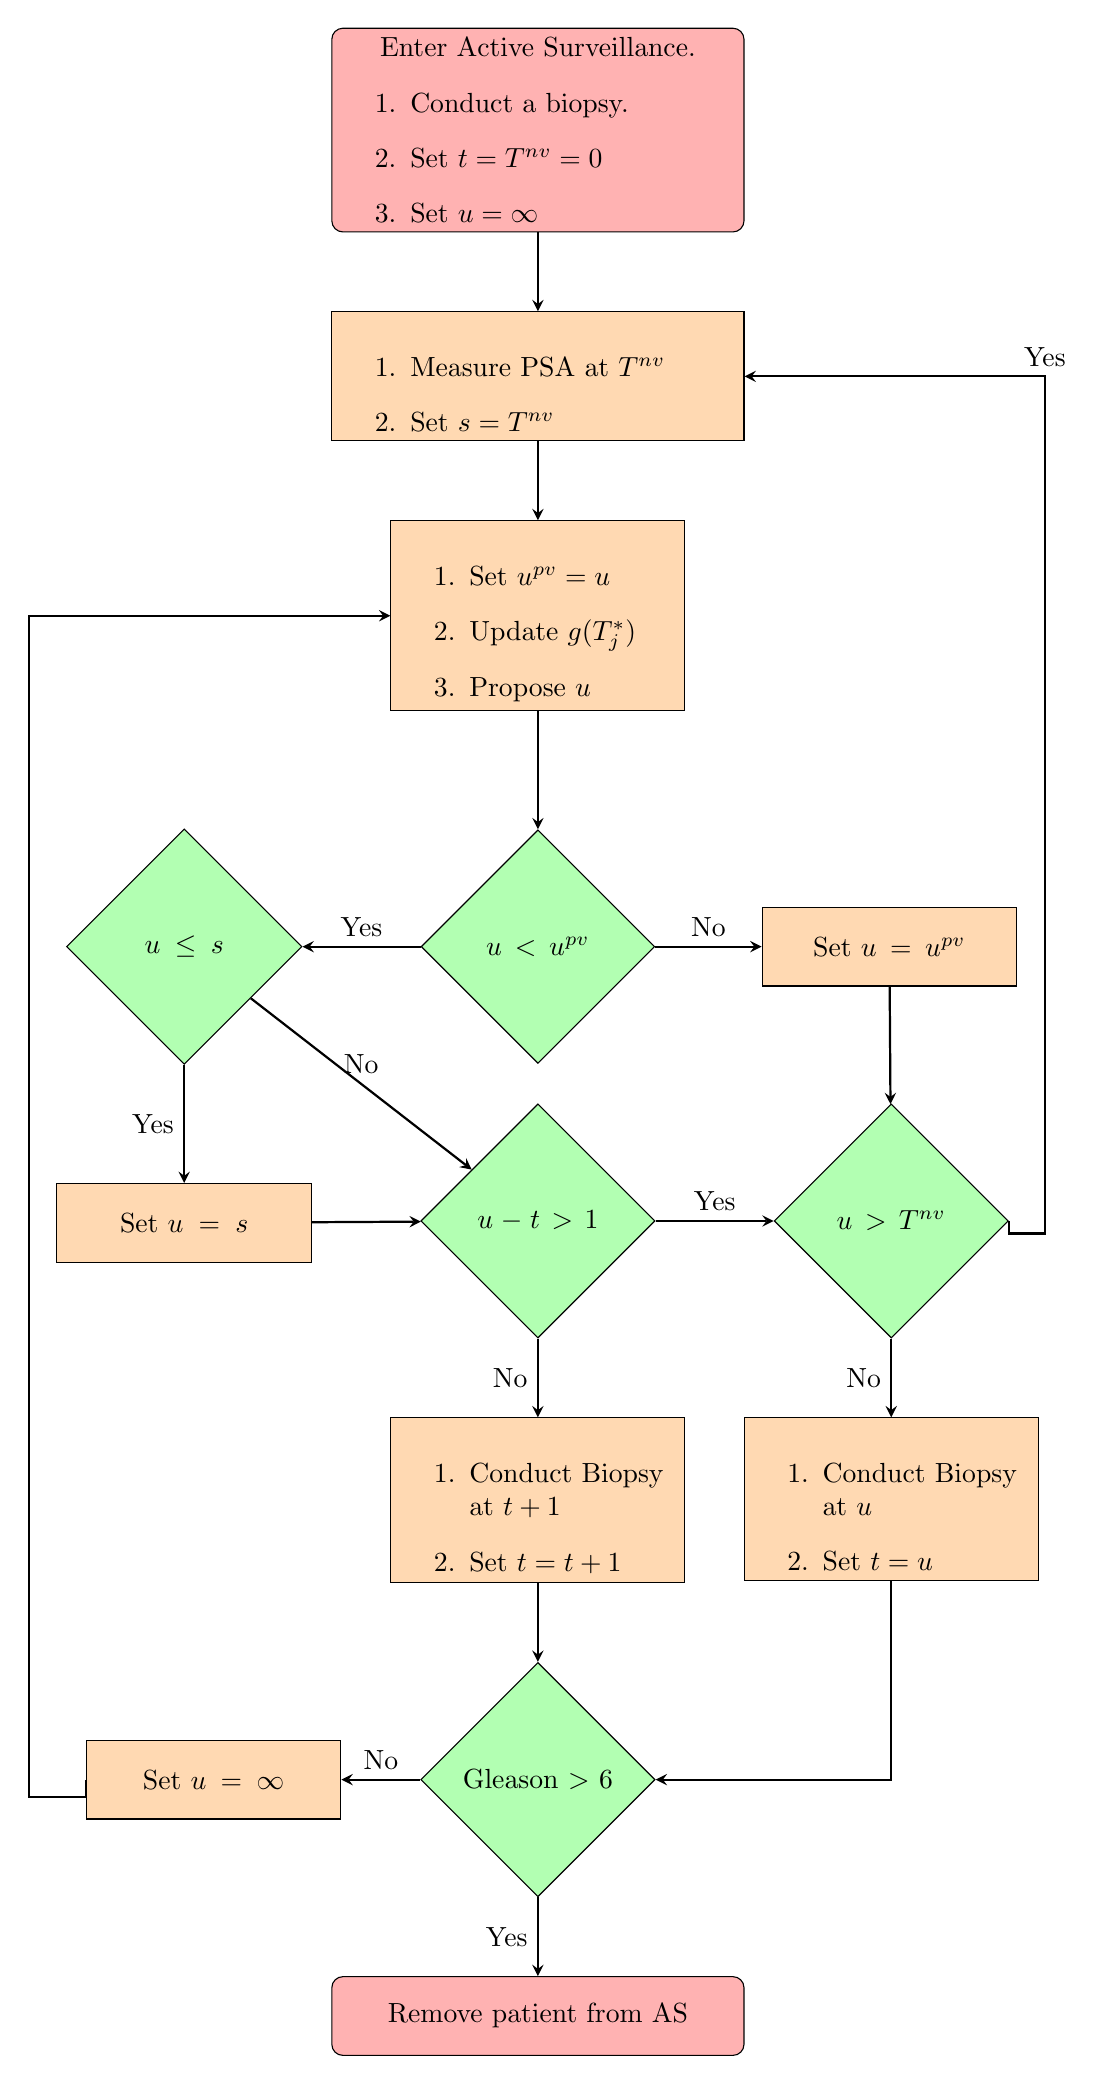
\begin{tikzpicture}
\node (start) [startstop] {
Enter Active Surveillance.
\begin{enumerate}
\item Conduct a biopsy.
\item Set $t=T^{nv}=0$ 
\item Set $u = \infty$
\end{enumerate}
};

\node (takePSA) [process_wide_5cm, below=1cm of start] {
\begin{enumerate}
\item Measure PSA at $T^{nv}$ 
\item Set $s=T^{nv}$
\end{enumerate}
};

\node (propTime) [process_wide_3pt5cm, below=1cm of takePSA] {
\begin{enumerate}
\item Set $u^{pv} = u$ 
\item Update $g(T^*_j)$ 
\item Propose $u$
\end{enumerate}
};

\node (decision1) [decision, below = 1.5cm of propTime] {$u < u^{pv}$};
\node (pro6) [process, right = 1.35cm of decision1] {Set $u = u^{pv}$};

\node (decision5) [decision, left=1.5cm of decision1] {$u \leq s$};

\node (pro5) [process, below=1.5cm of decision5] {Set $u = s$};

\node (decision2) [decision, below=0.5cm of decision1] {$u - t > 1$};

\node (decision4) [decision, right=1.5cm of decision2] {$u > T^{nv}$};

\node (pro3) [process_wide_3pt5cm, below=1cm of decision2] {
\begin{enumerate}
\item Conduct Biopsy at $t + 1$ 
\item Set $t = t + 1$
\end{enumerate}
};

\node (pro4) [process_wide_3pt5cm, below=1cm of decision4] {
\begin{enumerate}
\item Conduct Biopsy at $u$
\item Set $t = u$
\end{enumerate}
};

\node (decision3) [decision, below=1cm of pro3] {$\mbox{Gleason} > 6$};
\node (pro7) [process, left=1cm of decision3] {Set $u=\infty$};

\node (stop) [startstop, below = 1cm of decision3] {Remove patient from AS};

\draw [arrow] (start) -- (takePSA);
\draw [arrow] (takePSA) -- (propTime);
\draw [arrow] (propTime) -- (decision1);
\draw [arrow] (decision1) -- node[anchor=south] {Yes} (decision5);
\draw [arrow] (decision5) -- node[anchor=east] {Yes} (pro5);
\draw [arrow] (pro5) -- (decision2);
\draw [arrow] (decision1) -- node[anchor=south] {No} (pro6);
\draw [arrow] (decision5) -- node[anchor=south] {No} (decision2);
\draw [arrow] (pro6) -- (decision4);
\draw [arrow] (decision4.east) |- ([xshift=0.35cm, yshift=-4.15cm]pro6.north east) |- node[anchor=south] {Yes} (takePSA);
\draw [arrow] (decision2) -- node[anchor=south] {Yes} (decision4);
\draw [arrow] (decision2) -- node[anchor=east] {No} (pro3);
\draw [arrow] (pro3) -- (decision3);
\draw [arrow] (pro4) |- (decision3);
\draw [arrow] (decision3) -- node[anchor=east] {Yes} (stop);
\draw [arrow] (decision4) -- node[anchor=east] {No} (pro4);
\draw [arrow] (decision3) -- node[anchor=south]{No} (pro7);
\draw [arrow] (pro7.west)|- ([xshift=-0.35cm, yshift=-7.8cm]pro5.north west) |- (propTime);
\end{tikzpicture}

}%

}
%\caption{Algorithm for creating a personalized schedule for patient $j$. The time of the latest biopsy is denoted by $t$. The time of the latest available PSA measurement is denoted by $s$. The proposed personalized time of biopsy is denoted by $u$.  The time at which a repeat biopsy was proposed on the last visit to the hospital is denoted by $u^{pv}$. The time of the next visit for the measurement of PSA is denoted by $T^{nv}$.} 
%\end{figure}

\begin{figure*}
\label{fig : sched_algorithm}
\centerline{\resizebox{2\columnwidth}{!}{
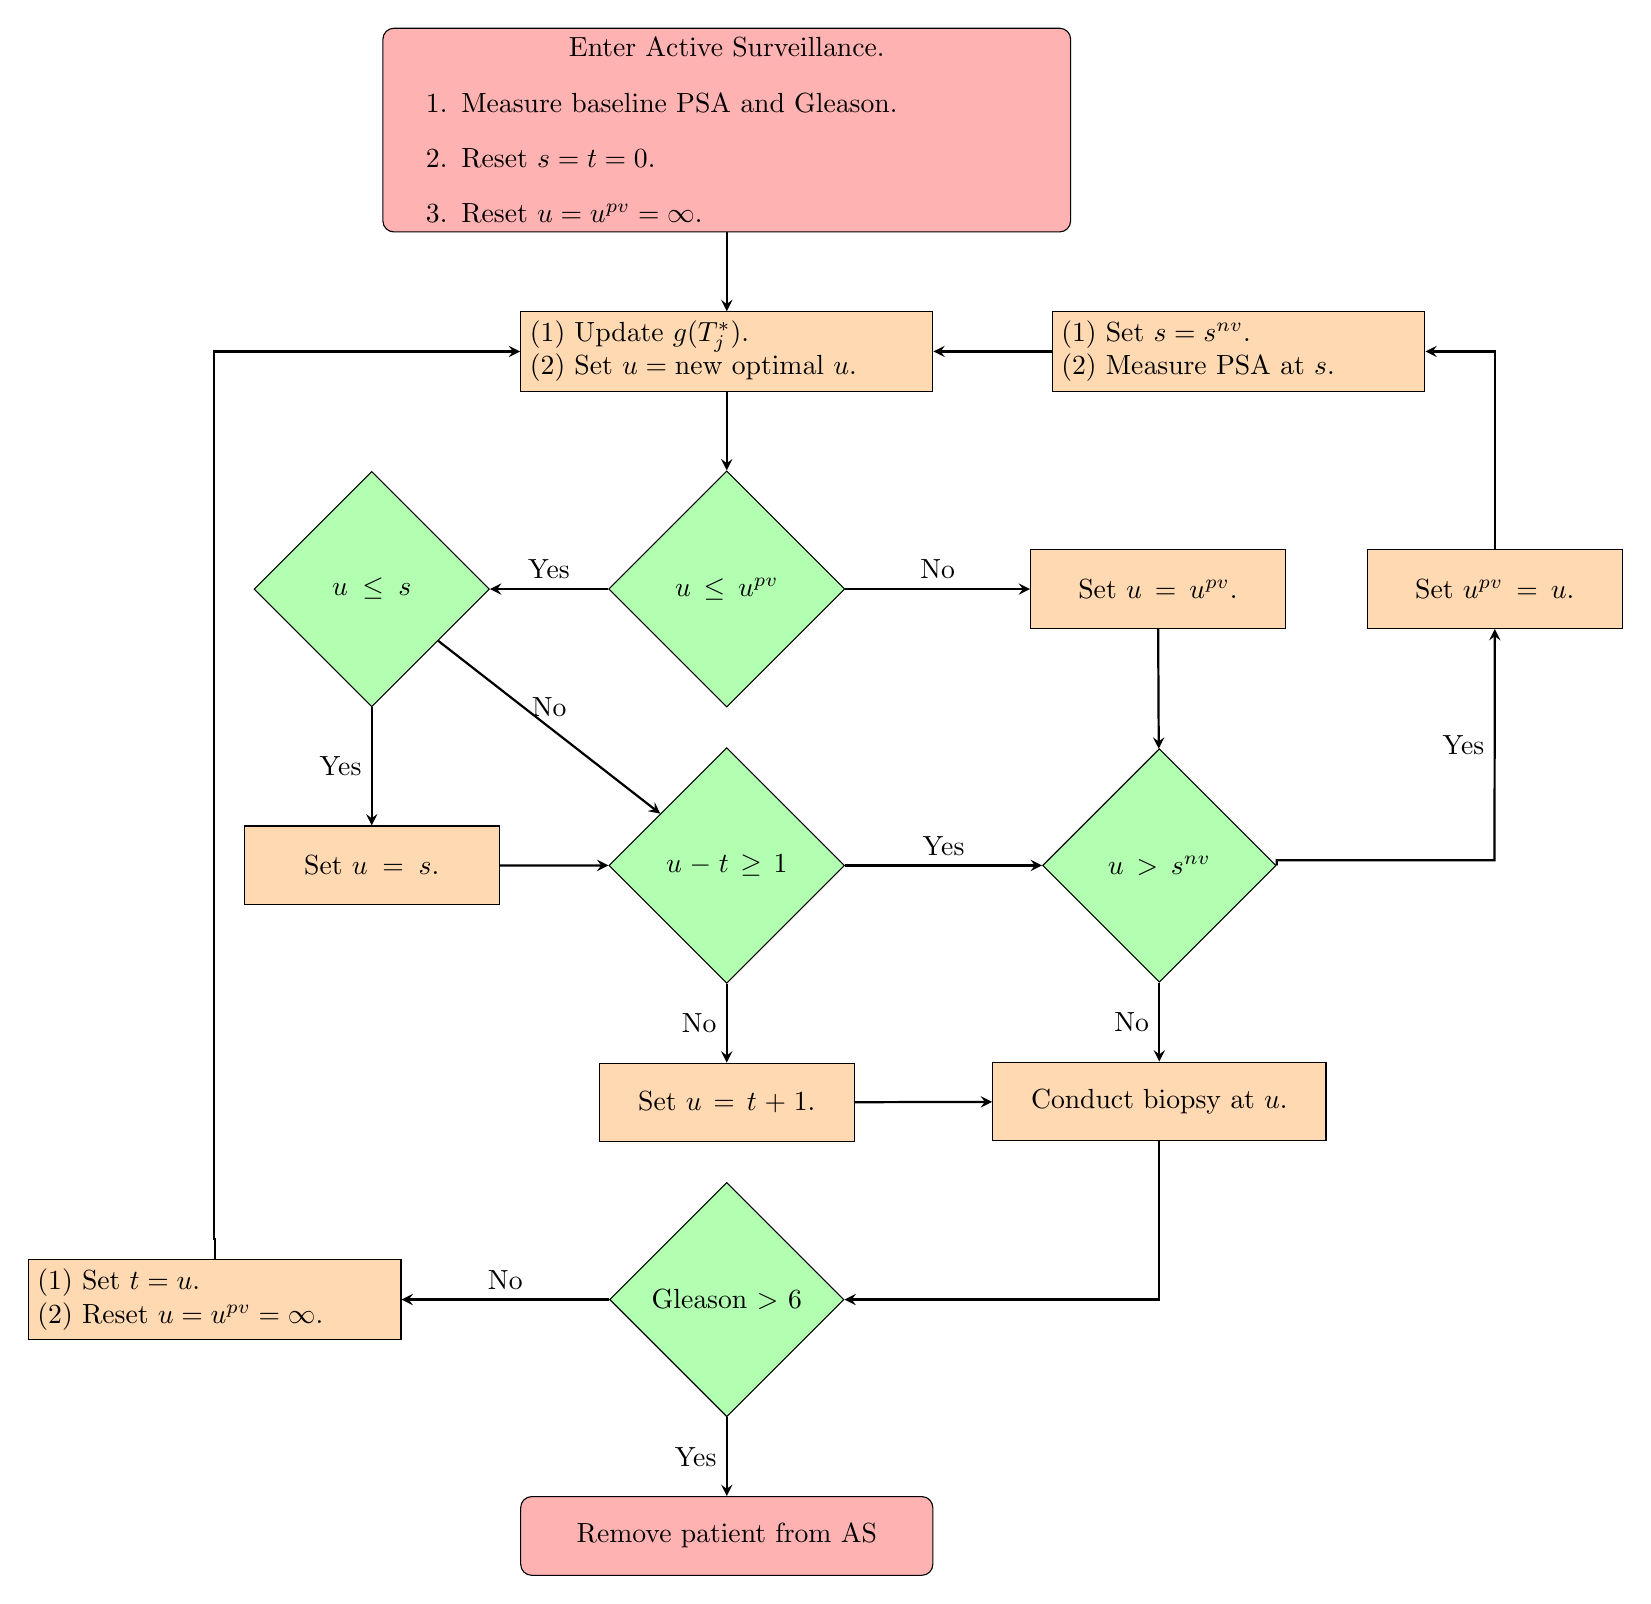
\begin{tikzpicture}
\node (start) [startstop_big] {
Enter Active Surveillance.
\begin{enumerate}
\item Measure baseline PSA and Gleason.
\item Reset $s=t=0$. 
\item Reset $u = u^{pv} = \infty$.
\end{enumerate}
};

\node (propTime) [process_wide_5cm, below=1cm of start] {
(1) Update $g(T^*_j)$.\\
(2) Set $u = \mbox{new optimal } u$.
};

\node (decision1) [decision, below = 1.0cm of propTime] {$u \leq u^{pv}$};
\node (pro6) [process, right = 2.345cm of decision1] {Set $u = u^{pv}$.};

\node (takePSA) [process_wide_4pt5cm, right=1.5cm of propTime] {
(1) Set $s=s^{nv}$.\\
(2) Measure PSA at $s$. 
};


\node (decision5) [decision, left=1.5cm of decision1] {$u \leq s$};

\node (pro5) [process, below=1.5cm of decision5] {Set $u = s$.};

\node (decision2) [decision, below=0.5cm of decision1] {$u - t \geq 1$};

\node (decision4) [decision, right=2.5cm of decision2] {$u > s^{nv}$};

\node (pro8) [process, right=1.03cm of pro6] {Set $u^{pv}=u$.};

\node (pro3) [process, below=1.0cm of decision2] {Set $u = t + 1$.};

\node (pro4) [process_wide_4cm, below=1cm of decision4] {Conduct biopsy at $u$.};

\node (decision3) [decision, below=0.5cm of pro3] {$\mbox{Gleason} > 6$};
\node (pro7) [process_wide_4pt5cm, left=2.635cm of decision3] {
(1) Set $t = u$.\\
(2) Reset $u = u^{pv}=\infty$.
};

\node (stop) [startstop, below = 1cm of decision3] {Remove patient from AS};

\draw [arrow] (start) -- (propTime);
\draw [arrow] (takePSA) -- (propTime);
\draw [arrow] (propTime) -- (decision1);
\draw [arrow] (decision1) -- node[anchor=south] {Yes} (decision5);
\draw [arrow] (decision5) -- node[anchor=east] {Yes} (pro5);
\draw [arrow] (pro5) -- (decision2);
\draw [arrow] (decision1) -- node[anchor=south] {No} (pro6);
\draw [arrow] (decision5) -- node[anchor=south] {No} (decision2);
\draw [arrow] (pro6) -- (decision4);
\draw [arrow] (decision4.east) |- ([xshift=2.65cm, yshift=-3.95cm]pro6.north east) -- node[anchor=east] {Yes} (pro8);

\draw [arrow] (pro8) |- (takePSA);

\draw [arrow] (decision2) -- node[anchor=south] {Yes} (decision4);
\draw [arrow] (decision2) -- node[anchor=east] {No} (pro3);
\draw [arrow] (pro3) -- (pro4);
\draw [arrow] (pro4) |- (decision3);
\draw [arrow] (decision3) -- node[anchor=east] {Yes} (stop);
\draw [arrow] (decision4) -- node[anchor=east] {No} (pro4);
\draw [arrow] (decision3) -- node[anchor=south]{No} (pro7);
\draw [arrow] (pro7.north)|- ([xshift=-0.375cm, yshift=-5.25cm]pro5.north west) |- (propTime);
\end{tikzpicture}
}
}
\caption{Algorithm for creating a personalized schedule for patient $j$. $t$ denotes the time of the latest biopsy. $s$ denotes the time of the latest available PSA measurement. $u$ denotes the proposed personalized time of biopsy.  $u^{pv}$ denotes the time at which a repeat biopsy was proposed on the last visit to the hospital. $T^{nv}$ denotes the time of the next visit for measurement of PSA.} 
\end{figure*}
% !TEX root =  ../pers_schedules.tex

\section{Choosing a Schedule}
\label{sec : choosing_schedule}
Given a particular schedule $S$ of biopsies, our next goal is to evaluate the efficacy of this schedule and to compare it with other schedules. To this end, we first present the criteria for evaluation of efficacy of biopsy schedules and then discuss the choice of the optimal schedule.

\subsection{Evaluation of Efficacy of Schedules}
We measure the efficacy of a schedule $S$ using two criteria, namely, for the $j$-th patient the number of biopsies $N^{bS}_j \epsilon [1, \infty]$ a schedule conducts before GR is detected, and the offset $O^S_j \epsilon [0, \infty]$ by which it overshoots the true GR time $T^*_j$. The offset $O^S_j$ is defined as $O^S_j = T^S_{j{N^{bS}_j}} - T^*_j$, where $T^S_{j{N^{bS}_j}} \geq T^*_j$ is the time at which GR is detected. Our interest lies in the joint distribution $p(N^{bS}_j, O^S_j)$ of the number of biopsies and the offset. Given the medical and financial burden associated with biopsies, ideally only one biopsy which leads to a zero offset should be conducted. That is, a method with a low mean number of biopsies $E(N^{bS}_j)$ as well a low mean offset $E(O^S_j)$ is desired. It is also desired that a method has low variance of the number of biopsies $\mbox{var}(N^{bS}_j)$, as well as low variance of the offset $\mbox{var}(O^S_j)$, so that the method works similarly for most patients. Quantiles of $p(N^{bS}_j)$ may also be of interest. For example, a schedule which conducts less than two biopsies in 95\% of the cases may be preferred.

\subsection{Finding the Optimal Schedule}
Given the multiple measures of efficacy of a schedule, the next step is to find the optimal schedule. Using principles from compound optimal designs \citep{lauter1976optimal} we propose to choose a schedule $S$ which minimizes a loss function of the following form:
\begin{equation}
\label{eq : loss_func_sim_study_generic}
L(S) = \sum_{r=1}^R \eta_r \mathcal{R}_r(N^{bS}_j).
\end{equation}
where $\mathcal{R}_r(\cdot)$ is a measure of efficacy of either the number of biopsies or the offset (in the equation above, only $N^{bS}_j$ is used for brevity of notation). Some examples of $\mathcal{R}_r(\cdot)$ are mean, median, variance and quantile function. Constants $\eta_1, \ldots, \eta_R$, where $\eta_r \epsilon [0,1]$ and $\sum_{r=1}^R \eta_r = 1$, are weights to differentially weigh-in the contribution of each of the $R$ measures of efficacy. An example loss function is:
\begin{equation}
\label{eq : loss_func_sim_study}
L(S) = \eta_1 E(N^{bS}_j) + \eta_2 E(O^S_j). 
\end{equation}
The choice of $\eta_1$ and $\eta_2$ is not easy, because biopsies have serious medical side effects and consequently the cost of an extra biopsy cannot be quantified or compared to a unit increase in offset easily. To obviate this problem we utilize the equivalence between compound and constrained optimal designs \citep{cook1994equivalence}. More specifically, it can be shown that for any $\eta_1$ and $\eta_2$ there exists a constant $C>0$ for which minimization of loss function in (\ref{eq : loss_func_sim_study}) is equivalent to minimization of the loss function subject to the constraint that $E(O^S_j) < C$. That is, the optimal schedule is the one with the least number of biopsies and an offset less than $C$. The choice of $C$ now can be based on the protocol of AS program. In the more generic case in (\ref{eq : loss_func_sim_study_generic}), the optimal solution can be found by minimizing $\mathcal{R}_R(\cdot)$ under the constraint $\mathcal{R}_r(\cdot) < C_r; r=1, \ldots, R-1$.
% !TEX root =  ../pers_schedules.tex

\section{Personalized schedules for patients in PRIAS}
\label{sec : pers_schedule_PRIAS}
To demonstrate how the personalized schedules work, we apply them to the patients enrolled in PRIAS. To this end, we divide the PRIAS dataset into a training data set with 5264 patients and a demonstration dataset with 3 patients who never experienced GR. We fit a joint model to the training dataset and then use it to create personalized schedules for patients in demonstration dataset. We fit the joint model using the R package JMbayes \citep{rizopoulosJMbayes}, which uses the Bayesian methodology to estimate the model parameters.

\subsection{Fitting the joint model to PRIAS dataset}
\label{subsec : jm_fit_prias}
The training dataset contains PSA levels and the time interval in which GR was detected, for 5264 prostate cancer patients. For every patient the following information is available: age at the time of induction, PSA at every 3 months for first 2 years and every 6 months thereafter. To detect GR, biopsies were conducted as per the PRIAS schedule(Section \ref{sec : introduction}). For the longitudinal analysis of PSA we use $\log_2 \mbox{PSA}$ measurements instead of the raw data. This because the PSA scores take very large values around the time of disease progression, indicating that the underlying distribution for PSA is right skewed. The longitudinal sub-model of the joint model we fit is given by:
\begin{equation}
\label{eq : long_model_prias}
\begin{aligned}
\log_2 \mbox{PSA}(t) &= \beta_0 + \beta_1 (Age-70) + \beta_2 (Age-70)^2 + \sum_{k=1}^4 \beta_{k+2} B_k(t,\mathcal{K})\\ 
&+  b_{i0} + b_{i1} B_7(t, 0.1) + b_{i2} B_8(t, 0.1) +
\varepsilon_i(t)
\end{aligned}
\end{equation}
The evolution of PSA over time is modeled flexibly using B-splines. The spline for the fixed effects consists of 3 internal knots at $\mathcal{K} =\{0.1, 0.5, 4\}$ years, and boundary knots at 0 and 7 years. The spline for the random effects consists of 1 internal knot at 0.1 years and boundary knots at 0 and 7 years. The choice of knots was based on exploratory analysis as well as on model selection criteria AIC and BIC. Age of patients was median centered to avoid numerical instabilities during parameter estimation. For the relative risk sub-model the hazard function we fit is given by:
\begin{equation}
\label{eq : hazard_prias}
h_i(t) = h_0(t) \exp\big[\gamma_1 \{Age-70\}  + \gamma_2 \{Age-70\}^2 + \alpha_1 m_i(t) + \alpha_2 m'_i(t)\big]
\end{equation}
where $\alpha_1$ and $\alpha_2$ are measures of strength of the association between hazard of GR and $\log_2 \mbox{PSA}$ value $m_i(t)$ and $\log_2 \mbox{PSA}$ velocity $m'_i(t)$, respectively. Since the PRIAS schedule depends only on the observed PSA values (via PSA-DT), the interval censoring observed in PRIAS is independent and non informative of the underlying health of the patient.

From the joint model fitted to the PRIAS dataset we found that only $\log_2 \mbox{PSA}$ velocity was strongly associated with hazard of GR. For any patient, a unit increase in $\log_2 \mbox{PSA}$ velocity led to an 11 times increase in the hazard of GR. The parameter estimates for the fitted joint model are presented in detail in Section 3 of the supplementary material. 

\subsection{Demonstration of personalized schedules}
\label{subsec : demo_prias_pers_schedule}
Using the demonstration dataset, we next present the functioning of personalized schedules based on expected time of GR and dynamic risk of GR. The first patient of interest is patient 3174. The PPD $g(T^*_j)$ for this patient depends only on the PSA levels since no repeat biopsies were conducted in the time period we considered. The evolution of PSA, repeat biopsy history and proposed times of biopsies are shown in Figure \ref{fig : prias_demo_pid_3174}. It can be seen that the schedule of biopsy based on expected time of GR adjusts the times of biopsy according to the rise in hazard due steep rise in $\log_2 \mbox{PSA}$ velocity after year 2. More specifically, at 2 years the proposed biopsy time is 12.5 years whereas at 4 years it decreases to 5.3 years. A biopsy scheduled using expected time of GR at year 2 should have a larger offset $O^S_j$ on average compared to the same at year 4. This because $\mbox{var}_g[T^*_j]$ is considerably lower at year 4 as shown in Figure \ref{fig : variance_pred_dist_3174_911}. As expected the variance also strongly depends on PSA velocity. For schedules based on dynamic risk of GR, the optimal $1 - \kappa$ value was found to be between 0 and 0.1 at all time points. Due to the sharp rise in PSA values, this corresponds to a time very close to the time of latest biopsy (time 0). Hence the biopsies are scheduled much earlier than those based on expected time of GR. 

\begin{figure}
\centerline{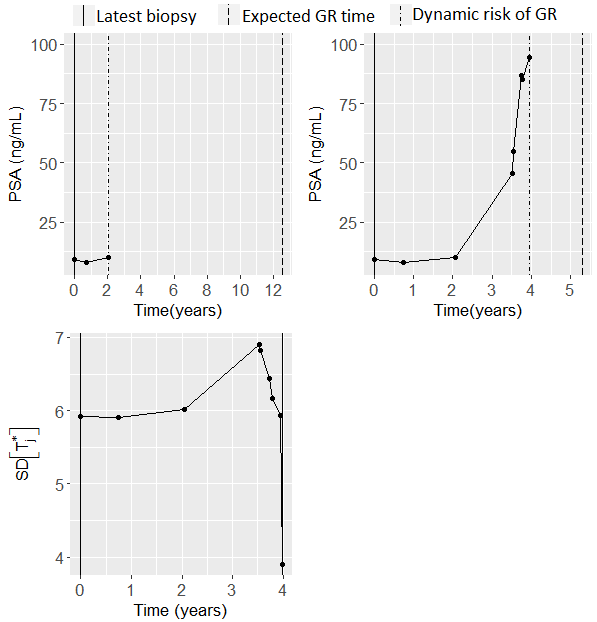
\includegraphics[width=\columnwidth]{images/prias_demo/case_3174.png}}
\caption{PSA and repeat biopsy history, and corresponding personalized schedules for patient 3174.}
\label{fig : prias_demo_pid_3174}
\end{figure}

\begin{figure}
\centerline{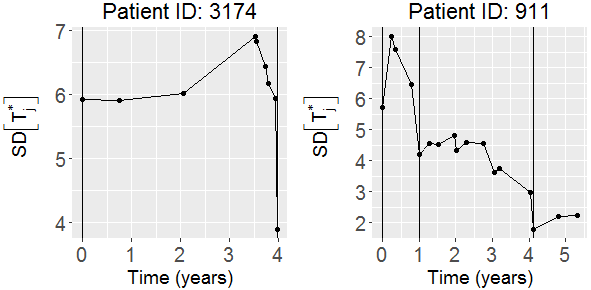
\includegraphics[width=\columnwidth]{images/prias_demo/variance_3174_911.png}}
\caption{Standard deviation $\mbox{SD}[T^*_j] = \sqrt{\mbox{var}_g[T^*_j]}$ over time for patient 3174 and 911. Solid vertical lines indicate biopsies.}
\label{fig : variance_pred_dist_3174_911}
\end{figure}

The second patient of interest is patient 911, for whom the evolution of PSA, time of last biopsy and proposed biopsy times are shown in Figure \ref{fig : prias_demo_pid_911}. We can see the combined effect of decreasing PSA levels and a negative repeat biopsy on personalized schedules, between year 3 and year 4.5 for this patient. In accordance with the observed history of the patient, the proposed time of biopsy based on expected time of GR increases from 16.6 years to 18.7 years in this period. For dynamic risk of GR it increases from 3.2 years to 15 years, despite the optimal $\kappa$ being equal to 0.98 for the entire period. We can also see that after each repeat biopsy $\mbox{var}_g[T^*_j]$ decreases sharply (Figure \ref{fig : variance_pred_dist_3174_911}), thus in turn reducing the offset as well.

\begin{figure}
\centerline{
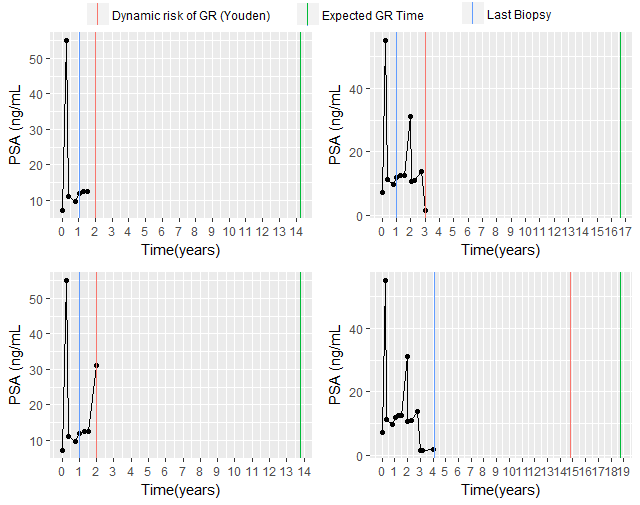
\includegraphics[width=\columnwidth]{images/prias_demo/case_911.png}
}
\caption{PSA and repeat biopsy history, and corresponding personalized schedules for patient 911.}
\label{fig : prias_demo_pid_911}
\end{figure}

Patient 2340 presents a case where information from PSA levels and repeat biopsies is conflicting. In Figure \ref{fig : prias_demo_pid_2340} we can see that the PSA for this patient becomes twice between year 2 and year 3.2. If only information from PSA is considered, then we can see that proposed time of biopsy based on expected time of GR is preponed from 12.5 to 11.5 years during this period. However, if we also take into account the negative result from the repeat biopsy at year 2.5, then the proposed time of biopsy is postponed from 12.5 years to 15 years. The proposed time of biopsy based on dynamic risk of GR is also preponed.

\begin{figure}
\centerline{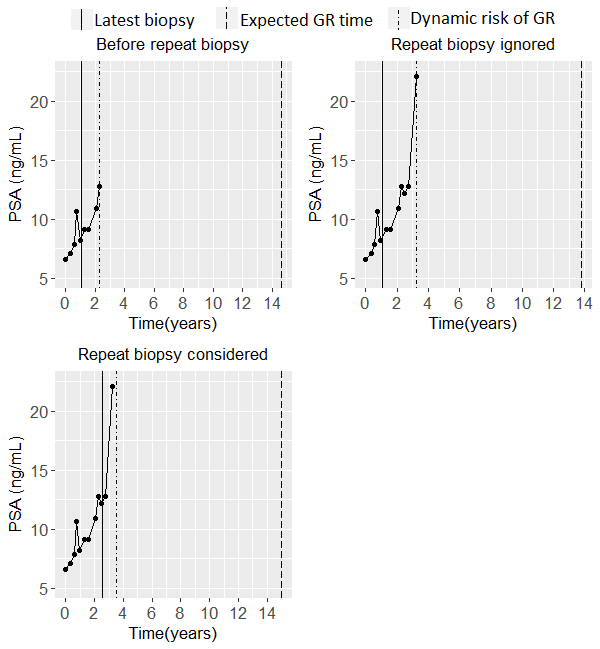
\includegraphics[width=\columnwidth]{images/prias_demo/case_2340.png}}
\caption{PSA and repeat biopsy history, and corresponding personalized schedules for patient 2340.}
\label{fig : prias_demo_pid_2340}
\end{figure}
% !TEX root =  ../main_manuscript.tex 
\section{Simulation Study}
\label{sec: simulation_study}
In Section \ref{subsec : demo_prias_pers_schedule} we demonstrated that the personalized schedules, schedule future biopsies according to the historical data of each patient. However, we could not perform a full-scale comparison between personalized and PRIAS schedules, because the true time of GR was not known for the PRIAS patients. To this end, we conducted a simulation study comparing personalized schedules with PRIAS and annual schedule, whose details are presented next.

\subsection{Simulation Setup}
\label{subsec : simulation_setup}
The population of AS patients in this simulation study is assumed to have the same entrance criteria as that of PRIAS. The PSA and hazard of GR for these patients follow a joint model of the form postulated in Section \ref{subsec : jm_fit_prias}, with parameters equal to the posterior mean of parameters estimated from the joint model fitted to the PRIAS dataset (see Web Appendix C). Furthermore, we also intend to test the efficacy of different schedules for a population which has patients with both faster as well as slowly-progressing PCa. The rate of progression is not only manifested via PSA profiles but also via the baseline hazard. We assume that there are three equal sized subgroups $G_1$, $G_2$ and $G_3$ of patients in the population, each with a baseline hazard from a Weibull distribution, with the following shape and scale parameters $(k, \lambda$): $(1.5, 4)$, $(3, 5)$ and $(4.5, 6)$ for $G_1, G_2$ and $G_3$, respectively. The effect of these parameters is that the mean GR time is lowest in $G_1$ (fast PCa progression) and highest in $G_3$ (slow PCa progression).

From this population, we have sampled 500 datasets with 1000 patients each. We generate a true GR time for each of the patients, and then sample a set of PSA measurements at the same time points as given in PRIAS protocol (see Web Appendix C). We then split the dataset into a training (750 patients) and a test (250 patients) part, and generate a random and non-informative censoring time for the training patients. We next fit a joint model of the specification given in (\ref{eq : long_model_prias}) and (\ref{eq : hazard_prias}) to each of the 500 training datasets and obtain MCMC samples from the 500 sets of the posterior distribution of the parameters. Using these fitted joint models, we obtain the posterior predictive distribution of time of GR for each of the $500 \times 250$ test patients. This distribution is further used to create personalized biopsy schedules for the test patients. For every test patient we conduct hypothetical biopsies using the following six types of schedules (abbreviated names in parenthesis): personalized schedules based on expected time of GR (Exp. GR time) and median time of GR (Med. GR time), personalized schedules based on dynamic risk of GR (Dyn. risk GR), a hybrid approach between median time of GR and dynamic risk of GR (Hybrid), PRIAS schedule and the annual schedule. The biopsies are conducted as per the algorithm in Figure \ref{fig : sched_algorithm}. 

To compare the aforementioned schedules we require estimates of the various measures of efficacy described in Section \ref{sec : choosing_schedule}. To this end, for schedule $S$, we compute pooled estimates of mean offset $E(O^S_j)$ and variance of offset $\mbox{var}(O^S_j)$, as below (estimates for $N^S_j$ are similar):
\begin{align*}
\widehat{E(O^S_j)} &= \frac{\sum_{k=1}^{500} n_k \widehat{E(O^S_k)}}{\sum_{k=1}^{500} n_k}, \\
\widehat{\mbox{var}(O^S_j)} &= \frac{\sum_{k=1}^{500} (n_k - 1) \widehat{\mbox{var}(O^S_k)}}{\sum_{k=1}^{500} (n_k-1)}, 
\end{align*}
where $n_k$ denotes the number of test patients, $\widehat{E(O^S_k)} = {\sum_{l=1}^{n_k}O^S_{kl}}/{n_k}$ is the estimated mean and $\widehat{\mbox{var}(O^S_k)} = {\sum_{l=1}^{n_k}\big\{O^S_{kl} - \widehat{E(O^S_k)}\big\}^2}/(n_k-1)$ is the estimated variance of the offset for the $k$-th simulation. The offset for the $l$-th test patient of the $k$-th dataset is denoted by $O^S_{kl}$.

\subsection{Results}
The pooled estimates of the aforementioned measures are summarized in Table \ref{table : sim_study_pooled_estimates}. In addition, estimated values of $E(O^S_j)$ are plotted against $E(N^S_j)$ in Figure \ref{fig : meanNbVsOffset}. The figure shows that across the schedules there is an inverse relationship between number $E(O^S_j)$ and $E(N^S_j)$. For example, the annual schedule conducts on average 5.2 biopsies to detect GR, which is the highest among all schedules. However, it has the least average offset of 6 months as well. On the other hand, the schedule based on expected time of GR conducts only 1.9 biopsies on average to detect GR, the least among all schedules, but it also has the highest average offset of 15 months (similar for median time of GR). Since the annual schedule attempts to contain the offset within a year it has the least $\mbox{SD}(O^S_j) = \sqrt{\mbox{var}(O^S_j)}$. However to achieve this, it conducts a wide range of number of biopsies from patient to patient, i.e., highest $\mbox{SD}(N^S_j) = \sqrt{\mbox{var}(N^S_j)}$. In this regard, schedules based on expected and median time of GR perform the opposite of annual schedule.

\begin{figure}
\centerline{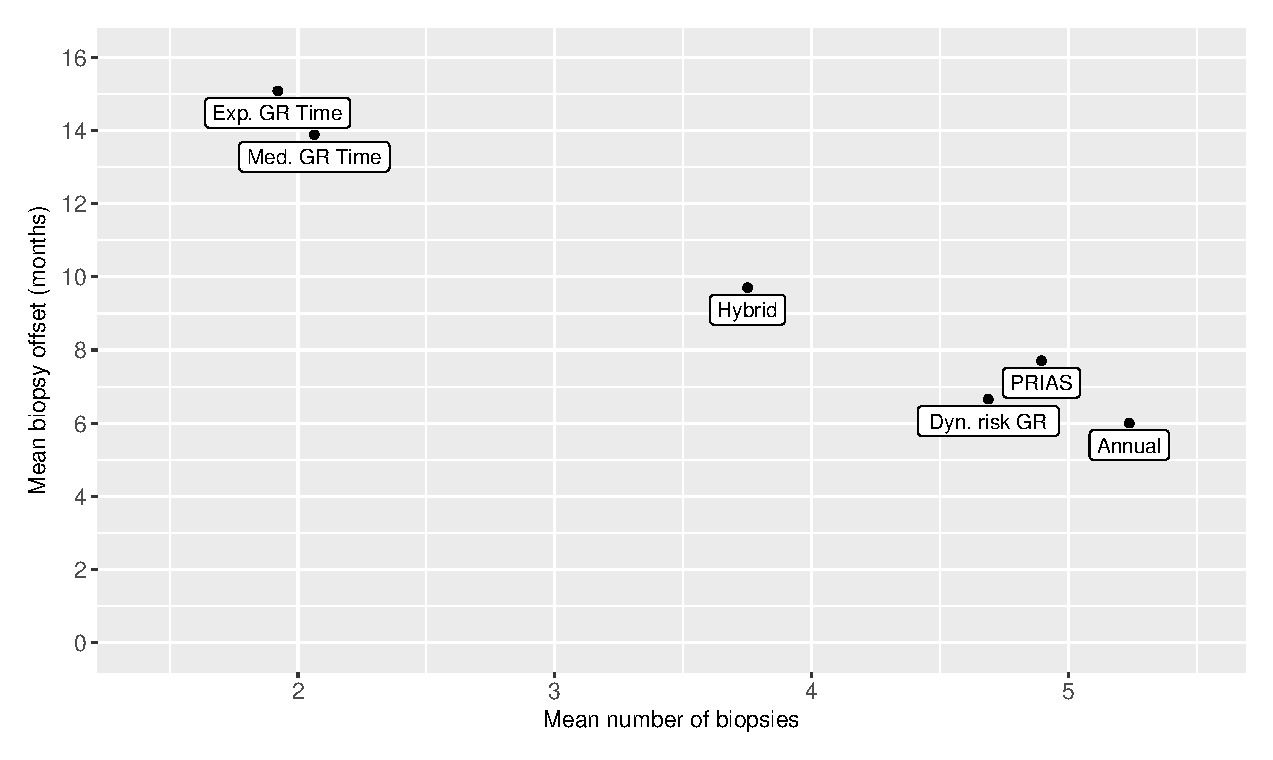
\includegraphics[width=\columnwidth]{images/sim_study/meanNbVsOffset_all.eps}}
\caption{Estimated mean number of biopsies and mean offset (months) for various schedules, obtained from the simulation study with 500 simulated datasets.}
\label{fig : meanNbVsOffset}
\end{figure}

%124781 = 41484 + 41423 + 41874
\begin{table}
\caption{Estimated mean and standard deviation of the number of biopsies $N^S_j$ and offset $O^S_j$ (months) for various schedules, obtained from the simulation study with 500 simulated datasets.}
\label{table : sim_study_pooled_estimates}
\begin{tabular}{lrrrr}
\Hline
\multicolumn{5}{c}{a) All hypothetical subgroups}\\
\hline
Schedule          & $E(N^S_j)$ & $E(O^S_j)$ & ${\mbox{SD}(N^S_j)}$ & ${\mbox{SD}(O^S_j)}$ \\
\hline
Annual         & 5.24            & 6.01                & 2.53          & 3.46              \\
PRIAS          & 4.90            & 7.71                & 2.36          & 6.31\\
Dyn. risk GR       & 4.69            & 6.66                & 2.19           & 4.38              \\
Hybrid       & 3.75            & 9.70                & 1.71          & 7.25              \\
Med. GR time & 2.06            & 13.88               & 1.41          & 11.80              \\
Exp. GR time & 1.92            & 15.08               & 1.19          & 12.11             \\
\hline
\multicolumn{5}{c}{b) Hypothetical subgroup $G_1$}\\
\hline
Schedule        & $E(N^S_j)$ & $E(O^S_j)$ & ${\mbox{SD}(N^S_j)}$ & ${\mbox{SD}(O^S_j)}$ \\
\hline
Annual         & 4.32            & 6.02                & 3.13          & 3.44              \\
PRIAS          & 4.07            & 7.44                & 2.88          & 6.11    \\
Dyn. risk GR       & 3.85            & 6.75                & 2.69          & 4.44              \\
Hybrid       & 3.25            & 10.25               & 2.16          & 8.07              \\
Med. GR time & 1.84            & 20.66               & 1.76          & 14.62             \\
Exp. GR time & 1.72            & 21.65               & 1.47          & 14.75             \\
\hline      
\multicolumn{5}{c}{c) Hypothetical subgroup $G_2$}\\
\hline
Schedule        & $E(N^S_j)$ & $E(O^S_j)$ & ${\mbox{SD}(N^S_j)}$ & ${\mbox{SD}(O^S_j)}$ \\
\hline
Annual         & 5.18            & 5.98                & 2.13          & 3.47              \\
PRIAS          & 4.85            & 7.70                & 2.00          & 6.29        \\
Dyn. risk GR       & 4.63            & 6.66                & 1.82          & 4.37              \\
Hybrid       & 3.68            & 10.32                & 1.37          & 7.45              \\
Med. GR time & 1.89             & 12.33               & 1.16          & 9.44              \\
Exp. GR time & 1.77            & 13.54               & 0.98          & 9.83              \\
\hline      
\multicolumn{5}{c}{d) Hypothetical subgroup $G_3$}\\
\hline
Schedule        & $E(N^S_j)$ & $E(O^S_j)$ & ${\mbox{SD}(N^S_j)}$ & ${\mbox{SD}(O^S_j)}$ \\
\hline
Annual         & 6.20             & 6.02                & 1.76          & 3.46              \\
PRIAS          & 5.76             & 7.98                & 1.71         & 6.51        \\
Dyn. risk GR       & 5.58            & 6.58                & 1.56          & 4.33              \\
Hybrid       & 4.32            & 8.55                & 1.26          & 5.91              \\
Med. GR time & 2.45            & 8.70                & 1.15          & 6.32              \\
Exp. GR time & 2.27            & 10.09               & 0.99          & 7.47              \\
\hline     
\end{tabular}
\end{table}

The PRIAS schedule conducts only 0.3 biopsies less than the annual schedule, but with a higher $\mbox{SD}(O^S_j)$, early detection is not always guaranteed. In comparison, the dynamic risk of GR based schedule performs slightly better than the PRIAS schedule in all four criteria. The hybrid approach combines the benefits of methods with low $E(N^S_j)$ and $\mbox{SD}(N^S_j)$, and methods with low $E(O^S_j)$ and $\mbox{SD}(O^S_j)$. It conducts 1.5 biopsies less than the annual schedule on average and with a $E(O^S_j)$ of 9.7 months it detects GR within a year since its occurrence. Moreover, it has both $\mbox{SD}(N^S_j)$ and $\mbox{SD}(O^S_j)$ comparable to PRIAS.

The performance of each schedule differs for the three subgroups $G_1, G_2$ and $G_3$. The annual schedule remains the most consistent across subgroups in terms of the offset, but it conducts 2 extra biopsies for the subgroup $G_3$ (slowly-progressing PCa) than $G_1$ (faster-progressing PCa). The performance of schedule based on expected time of GR is the most consistent in terms of the number of biopsies but it detects GR a year later on average in subgroup $G_1$ than $G_3$. For the dynamic risk of GR based schedule and the hybrid schedule, the dynamics are similar to that of the annual schedule. Unlike the latter two schedules, the PRIAS schedule not only conducts more biopsies in $G_3$ than $G_1$ but also detects GR later in $G_3$ than $G_1$.

\begin{figure}[!htb]
\centerline{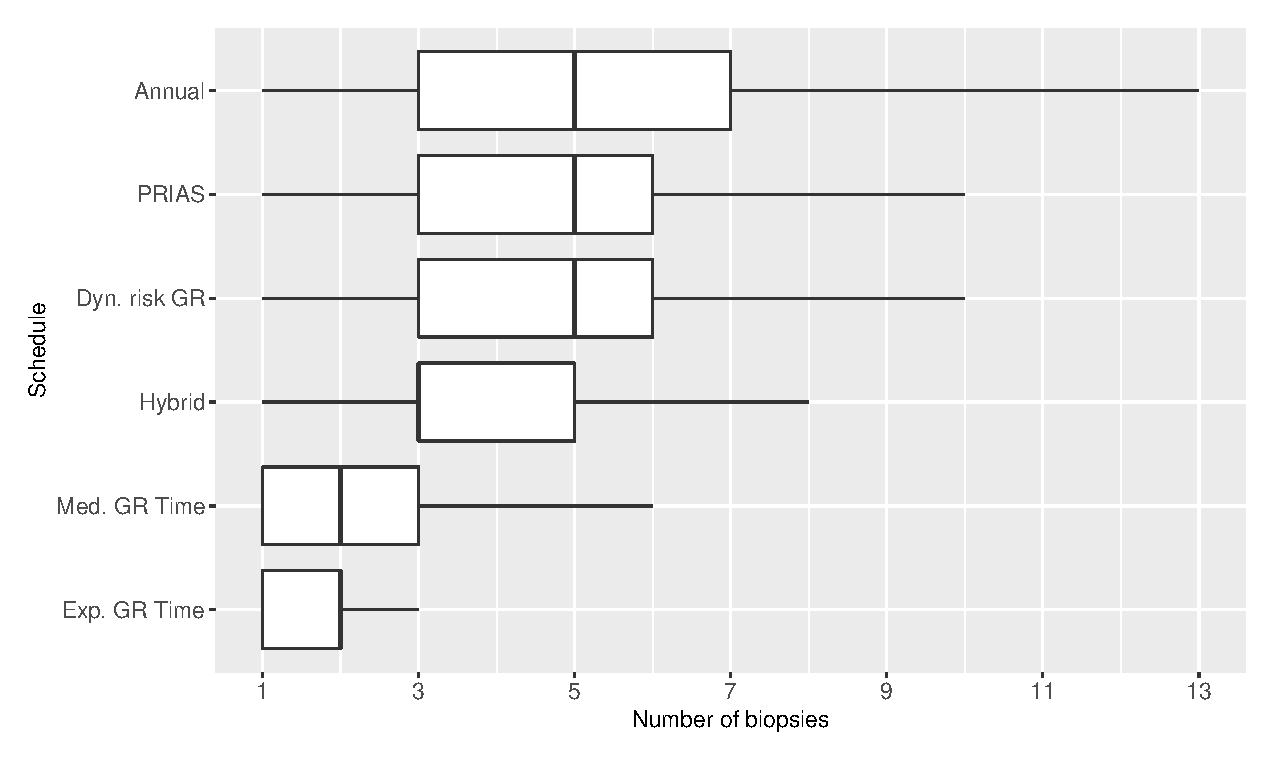
\includegraphics[width=\columnwidth]{images/sim_study/nbBoxPlot_all.eps}}
\caption{Boxplot showing variation in number of biopsies conducted by various schedules, obtained from the simulation study with 500 simulated datasets.}
\label{fig : nbBoxPlot_all}
\end{figure}

\begin{figure}[!htb]
\centerline{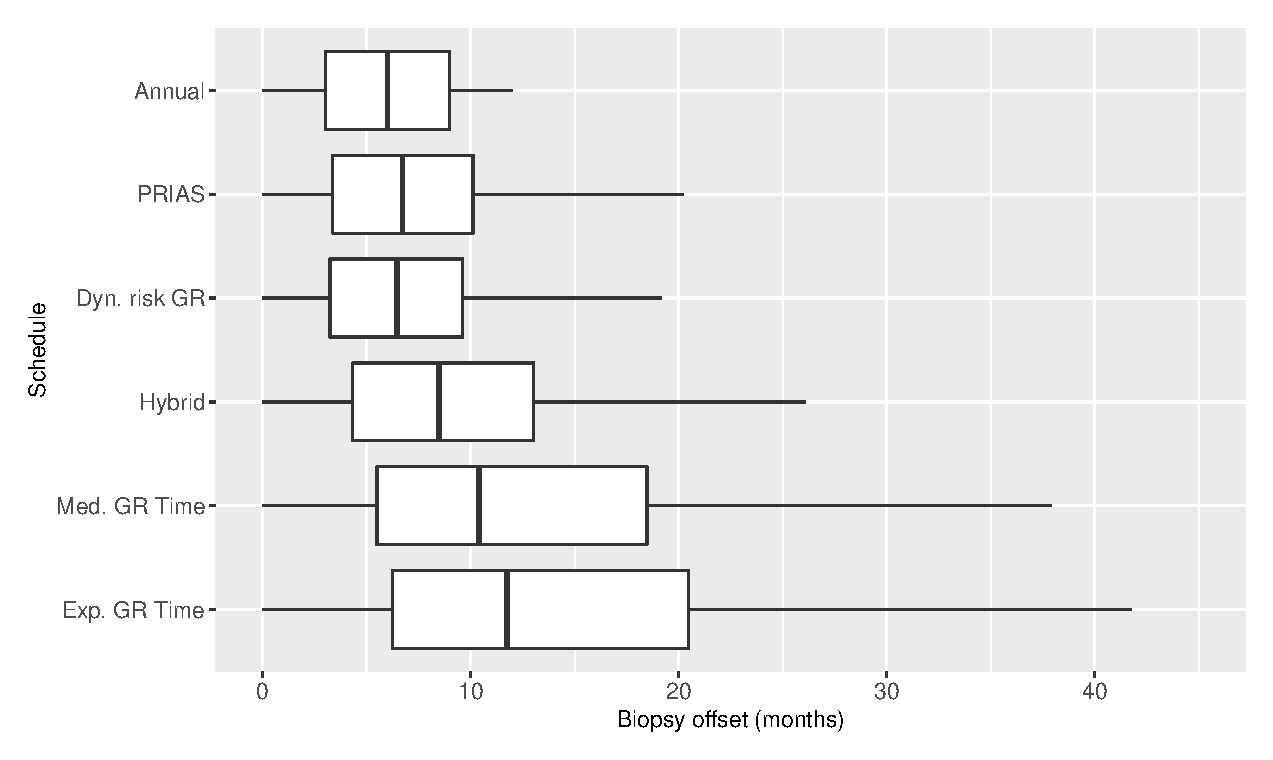
\includegraphics[width=\columnwidth]{images/sim_study/offsetBoxPlot_all.eps}}
\caption{Boxplot showing variation in biopsy offset (months) for various schedules, obtained from the simulation study with 500 simulated datasets.}
\label{fig : offsetBoxPlot_all}
\end{figure}

The choice of a suitable schedule using (\ref{eq : loss_func_sim_study_generic}) depends on the chosen measure for evaluation of schedules. In this regard, the schedules we compared either have high $\mbox{SD}(O^S_j)$ and low $\mbox{SD}(N^S_j)$, or vice versa (Table \ref{table : sim_study_pooled_estimates}). Thus, applying a cutoff on $E(O^S_j)$ when $\mbox{SD}(O^S_j)$ is high may not be as fruitful (same for $N^S_j$) as applying a cutoff on $\mbox{SD}(O^S_j)$ or quantile(s) of $O^S_j$. For example, the schedule based on the dynamic risk of GR is suitable if on average the least number of biopsies are to be conducted to detect GR, while simultaneously making sure that at least 90\% of the patients have an average offset less than one year.

% !TEX root =  ../main_manuscript.tex 
\section{Discussion}
\label{sec:discussion}
In this paper, we presented a methodology to create personalized schedules for burdensome diagnostic \textit{tests} utilized to detect disease \textit{progression} in early-stage chronic non-communicable disease \textit{surveillance}. For this purpose, we utilized joint models for time-to-event and longitudinal data. Our approach first combines a patient's clinical data (e.g., longitudinal biomarkers) and previous invasive test results to estimate patient-specific cumulative-risk of disease progression over their current and future follow-up visits. We then plan future invasive tests whenever this cumulative-risk of progression is predicted to be above a certain threshold. We select the risk threshold automatically in a personalized manner, by optimizing a utility function of the patient-specific consequences of choosing a particular risk threshold based schedule. These consequences are, namely, the number of invasive tests (burden) planned in a schedule, and the expected time delay in detection of progression (shorter is beneficial) if the patient progresses. Last, we calculate this expected time delay in a personalized manner for both personalized and fixed schedules to assist patients/doctors in making a more informed decision of choosing a test schedule.

Using joint models gives us certain advantages. First, since joint models employ random-effects, the corresponding risk-based schedules are inherently personalized. Second, to predict this patient-specific risk of progression, joint models utilize all observed longitudinal measurements of a patient. Also, the continuous longitudinal outcomes are not discretized, which is commonly a case in Markov Decision Process and flowchart-based test schedules. Third, personalized schedules update automatically with more patient data over follow-up. Fourth, we calculated the expected number of tests (burden) and expected time delay in detecting progression (shorter is beneficial) in a patient-specific manner. Using our methodology, these can be calculated for both personalized and fixed schedules. Thus, patients/doctors can compare risk-based and fixed schedules and choose one according to their preferences for the expected burden-benefit ratio. Last, although this work concerns invasive test schedules in disease surveillance, the methodology is generic for use under a screening setting as well.

Personalized schedules that we proposed require a risk threshold. We optimized the threshold choice using a generic utility function based on the expected number of biopsies and time delay in detecting progression. We used only these two measures because they are easy to interpret but simultaneously critical for deciding the timing of invasive tests. Also, the time delay in detecting progression should manifest the window of opportunity for curative treatment and additional benefits of observing progression early. Practitioners may extend/modify this utility function by adding to/replacing time delay with commonly used decision-theoretic measures such as quality-adjusted life-years/expectancy (QALY/QALE).

We evaluated personalized schedules in a full cohort via a realistic simulation of a randomized clinical trial for prostate cancer surveillance patients. We observed that personalized schedules reduced many unnecessary biopsies for non-progressing patients compared to the widely used annual schedule. This happened at the cost of simultaneously having a slightly more time delay in detecting progression. Although, this delay should still be safe because it was almost equal to the delay of the world's largest prostate cancer active surveillance program PRIAS's schedule. The simulation study results are by no means the performance-limit of the personalized schedules. Instead, models with higher predictive accuracy and discrimination capacity than the PRIAS based model may lead to an even better balance between the number of tests and the time delay in detecting progression.

There are certain limitations to this work. First, in practice, most cohorts have a limited study period. Hence, the cumulative-risk profiles of patients and resulting personalized schedules can only be created up to the maximum study period. For this problem, the risk prediction model should be updated with more follow-up data over time. The proposed joint model assumed all events other than progression to be non-informative censoring. Alternative models that account for competing risks may lead to better results as they estimate absolute and not the cause-specific risk of progression. Upgrading is susceptible to inter-observer variation and sampling error. Although models that account for these two issues~\citep{balasubramanian2003estimation,coley2017prediction} will provide better risk estimates, the methodology for obtained personalized schedules can remain the same.

%  The \backmatter command formats the subsequent headings so that they
%  are in the journal style.  Please keep this command in your document
%  in this position, right after the final section of the main part of 
%  the paper and right before the Acknowledgements, Supplementary Materials,
%  and References sections. 

\backmatter

%  This section is optional.  Here is where you will want to cite
%  grants, people who helped with the paper, etc.  But keep it short!

% !TEX root =  main_manuscript.tex

\section*{Acknowledgements}
The first and last authors would like to acknowledge support by the Netherlands Organization for Scientific Research's VIDI grant nr. 016.146.301, and Erasmus MC funding. The authors also thank the Erasmus MC Cancer Computational Biology Center for giving access to their IT-infrastructure and software that was used for the computations and data analysis in this study. Lastly, we thank Frank-Jan H. Drost from the Department of Urology, Erasmus University Medical Center, for helping us in accessing the PRIAS data set. \vspace*{-8pt}

%  If your paper refers to supplementary web material, then you MUST
%  include this section!!  See Instructions for Authors at the journal
%  website http://www.biometrics.tibs.org

\section*{Supplementary Materials}

Web Appendix A, C, D and E referenced in Section~\ref{sec : jm_framework},  Section~\ref{sec : pers_schedule_PRIAS},  and  Section~\ref{sec: discussion}, respectively, and the derivation of Equation (\ref{eq : expected_time_survprob}) and (\ref{eq : var_time_survprob}) in Web Appendix B, are available in the document supplementary\_material.pdf.\vspace*{-8pt}

%Web Appendix A and C, referenced in Section~\ref{sec : jm_framework} and  Section~\ref{sec : pers_schedule_PRIAS}  respectively, and the derivation of Equations ~\ref{eq : expected_time_survprob} and ~\ref{eq : var_time_survprob} in Web Appendix B, are available with
%this paper at the Biometrics website on Wiley Online Library.\vspace*{-8pt}

%  Here, we create the bibliographic entries manually, following the
%  journal style.  If you use this method or use natbib, PLEASE PAY
%  CAREFUL ATTENTION TO THE BIBLIOGRAPHIC STYLE IN A RECENT ISSUE OF
%  THE JOURNAL AND FOLLOW IT!  Failure to follow stylistic conventions
%  just lengthens the time spend copyediting your paper and hence its
%  position in the publication queue should it be accepted.

%  We greatly prefer that you incorporate the references for your
%  article into the body of the article as we have done here 
%  (you can use natbib or not as you choose) than use BiBTeX,
%  so that your article is self-contained in one file.
%  If you do use BiBTeX, please use the .bst file that comes with 
%  the distribution.  In this case, replace the thebibliography
%  environment below by 
%
%  \bibliographystyle{biom} 
% \bibliography{mybibilo.bib}

\bibliographystyle{biom} 
\bibliography{bibliography}

\appendix

%  To get the journal style of heading for an appendix, mimic the following.

%\section{}
%\subsection{Title of appendix}

%Put your short appendix here.  Remember, longer appendices are
%possible when presented as Supplementary Web Material.  Please 
%review and follow the journal policy for this material, available
%under Instructions for Authors at \texttt{http://www.biometrics.tibs.org}.

\label{lastpage}

\end{document}
